% Data Cluster presentation - Directorate for Education and Skills, OECD
% Build:  pdflatex main.tex  (run twice)
\documentclass[aspectratio=169,11pt]{beamer}

\usepackage[T1]{fontenc}
\usepackage{booktabs}
\usepackage{tikz}
\usetikzlibrary{decorations.pathreplacing,arrows.meta}

% ---------- look ----------
\usetheme{default}
\usefonttheme{serif}
\setbeamertemplate{navigation symbols}{}
\definecolor{navy}{HTML}{1F3864}
\definecolor{burg}{HTML}{7B2530}
\definecolor{ink}{HTML}{1A2430}
\definecolor{mut}{HTML}{6B7480}
\definecolor{paleblue}{HTML}{AFC3DC}
\setbeamercolor{frametitle}{fg=navy}
\setbeamercolor{title}{fg=navy}
\setbeamercolor{structure}{fg=navy}
\setbeamercolor{normal text}{fg=ink}
\setbeamerfont{frametitle}{series=\bfseries,size=\large}
\setbeamerfont{title}{series=\bfseries,size=\Large}
\setbeamertemplate{itemize item}{\textcolor{navy}{\footnotesize$\bullet$}}
\setbeamertemplate{itemize subitem}{\textcolor{mut}{\footnotesize--}}
\setbeamertemplate{footline}{%
  \hfill\textcolor{mut}{\scriptsize\insertframenumber}\hspace{2ex}\vspace{1ex}}
\setbeamersize{text margin left=0.9cm,text margin right=0.9cm}
\newcommand{\msg}[1]{{\color{navy}\bfseries #1}}

% ---------- NTPS 2020-21 comparison values (filled from NCES sources) ----------
\newcommand{\ntpsFemale}{76.8}
\newcommand{\ntpsMA}{61.0}
\newcommand{\ntpsAge}{42.9}
\newcommand{\ntpsN}{39,633}

\title{Measuring Teacher Attrition\\ with Labour Force Survey Data}
\subtitle{The Case of the United States}
\author{Jos\'e El\'ias Dur\'an Roa}
\institute{Data Cluster \,\textperiodcentered\, Directorate for Education and Skills}
\date{}
\titlegraphic{
\includegraphics[height=0.85cm]{oecd_logo.png}}

\begin{document}

\begin{frame}
  \titlepage
\end{frame}

% ================= A. Origin =================
\begin{frame}{Why this project}
  \vspace{1.2em}
  \begin{itemize}\setlength\itemsep{1.4em}
    \item Which of the factors we can observe correlate most strongly
          with the decision to leave teaching?
    \item Re-estimate the teacher leaving rate against the published
          figures of the official surveys.
  \end{itemize}
\end{frame}

% ================= Contribution =================
\begin{frame}{Contribution}
  \vspace{0.4em}
  \begin{enumerate}\setlength\itemsep{1.5em}
    \item \msg{A new series.} The longest \msg{continuous} series of teacher
          attrition to reach the present: one estimate for
          \msg{every year from 1997 to 2024}, constructed from twenty-eight
          consecutive supplements of the Current Population Survey.
    \item \msg{A measurement discussion.} A systematic treatment of the ways
          a longitudinal household survey identifies leaving: the linking of
          individuals across interviews, the alternative definitions of a
          leaver, and the assumptions each definition entails.
    \item \msg{Substantive evidence.} A characterization of who leaves
          teaching and of the observed factors most strongly associated with
          leaving, together with the destinations of leavers and the
          heterogeneity of attrition across states.
  \end{enumerate}
\end{frame}

% ================= B. Data =================
\begin{frame}{The CPS replicates the official picture --- and does it every year}
  \begin{center}
  \small
  \begin{tabular}{lccc}
    \toprule
                                   & CPS              & NTPS (official) & Difference \\
    \midrule
    Measurement                    & \msg{every year, 1997--2024}
                                   & occasional waves & \\
    \midrule
    \multicolumn{4}{l}{\color{mut}\footnotesize Example wave: 2020--21, the latest NTPS}\\[0.2em]
    Female (\%)                    & 75.5             & 76.8  & $-$1.3\phantom{$^{***}$}   \\
    Master's degree or higher (\%) & 57.0             & 61.0  & $-$4.0$^{***}$ \\
    Average age (years)            & 44.0             & 42.9  & $+$1.1$^{***}$ \\
    \midrule
    Teachers observed in the wave  & 3,855            & 39,633 & \\
    \bottomrule
  \end{tabular}
  \end{center}
  \vspace{0.5em}
  {\footnotesize\color{mut}
   Public school teachers. CPS: supplements of 2021--2022 (school years
   2020--21 and 2021--22), weighted. NTPS: National Teacher and Principal
   Survey 2020--21 (NCES 2022-113; Digest of Education Statistics,
   table 209.10; respondent count from NCES 2024-024). Stars test the CPS mean against the published NTPS estimate with design-adjusted standard errors: $^{***}$ $p<0.001$; the female share does not differ significantly.}
  \vspace{0.6em}

  {\small
   Full sample: \textbf{5.0 million} person-year records, 1998--2025;
   \textbf{104,545} teacher observations; \textbf{48,842} teachers followed
   across interviews in the linked panel.}
\end{frame}

% ================= C. CPS structure =================
\begin{frame}[plain]
  \begin{center}
  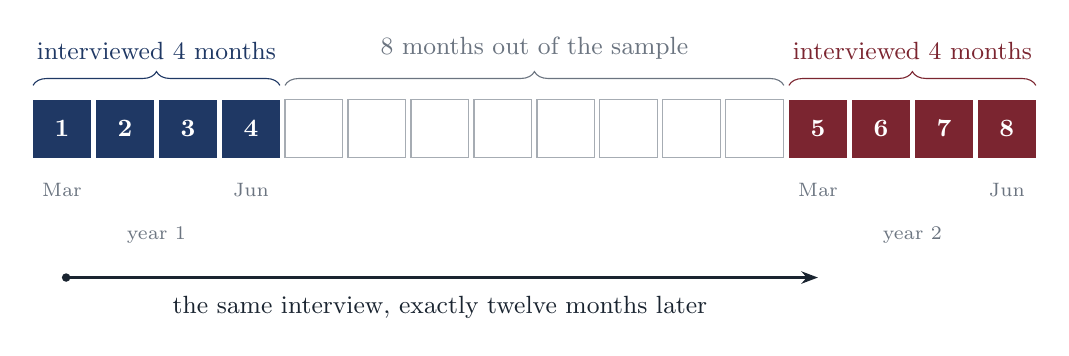
\begin{tikzpicture}[x=0.80cm,y=0.80cm]
    % month cells for one household: 4 in, 8 out, 4 in
    \foreach \i in {0,...,3}{
      \fill[navy] (\i,0) rectangle ++(0.92,0.92);
      \node[white,font=\small\bfseries] at (\i+0.46,0.46) {\the\numexpr\i+1};}
    \foreach \i in {4,...,11}{
      \draw[mut!60] (\i,0) rectangle ++(0.92,0.92);}
    \foreach \i in {12,...,15}{
      \fill[burg] (\i,0) rectangle ++(0.92,0.92);
      \node[white,font=\small\bfseries] at (\i+0.46,0.46) {\the\numexpr\i-7};}
    % month axis
    \node[anchor=north,font=\scriptsize,color=mut] at (0.46,-0.25) {Mar};
    \node[anchor=north,font=\scriptsize,color=mut] at (3.46,-0.25) {Jun};
    \node[anchor=north,font=\scriptsize,color=mut] at (12.46,-0.25) {Mar};
    \node[anchor=north,font=\scriptsize,color=mut] at (15.46,-0.25) {Jun};
    \node[anchor=north,font=\scriptsize,color=mut] at (1.96,-0.95) {year 1};
    \node[anchor=north,font=\scriptsize,color=mut] at (13.96,-0.95) {year 2};
    % braces
    \draw[decorate,decoration={brace,amplitude=5pt},navy]
      (0,1.15) -- (3.92,1.15) node[midway,above=6pt,font=\small\color{navy}]
      {interviewed 4 months};
    \draw[decorate,decoration={brace,amplitude=5pt},mut]
      (4,1.15) -- (11.92,1.15) node[midway,above=6pt,font=\small\color{mut}]
      {8 months out of the sample};
    \draw[decorate,decoration={brace,amplitude=5pt},burg]
      (12,1.15) -- (15.92,1.15) node[midway,above=6pt,font=\small\color{burg}]
      {interviewed 4 months};
    % twelve-month arrow
    \draw[{Circle[length=3pt]}-{Stealth[length=6pt]},thick,ink]
      (0.46,-1.9) -- (12.46,-1.9)
      node[midway,below=3pt,font=\small\color{ink}]
      {the same interview, exactly twelve months later};
  \end{tikzpicture}
  \end{center}
\end{frame}

\begin{frame}{The March supplement (ASEC)}
  \vspace{0.8em}
  \begin{itemize}\setlength\itemsep{1.2em}
    \item The largest supplement of the CPS: the March sample is expanded
          to roughly 90,000 households.
    \item Every adult reports on the \emph{previous calendar year}: longest
          job held, weeks worked, earnings, benefits.
    \item We use it to reconstruct the leaving rate.
  \end{itemize}
\end{frame}

\begin{frame}[plain]
  \begin{center}
    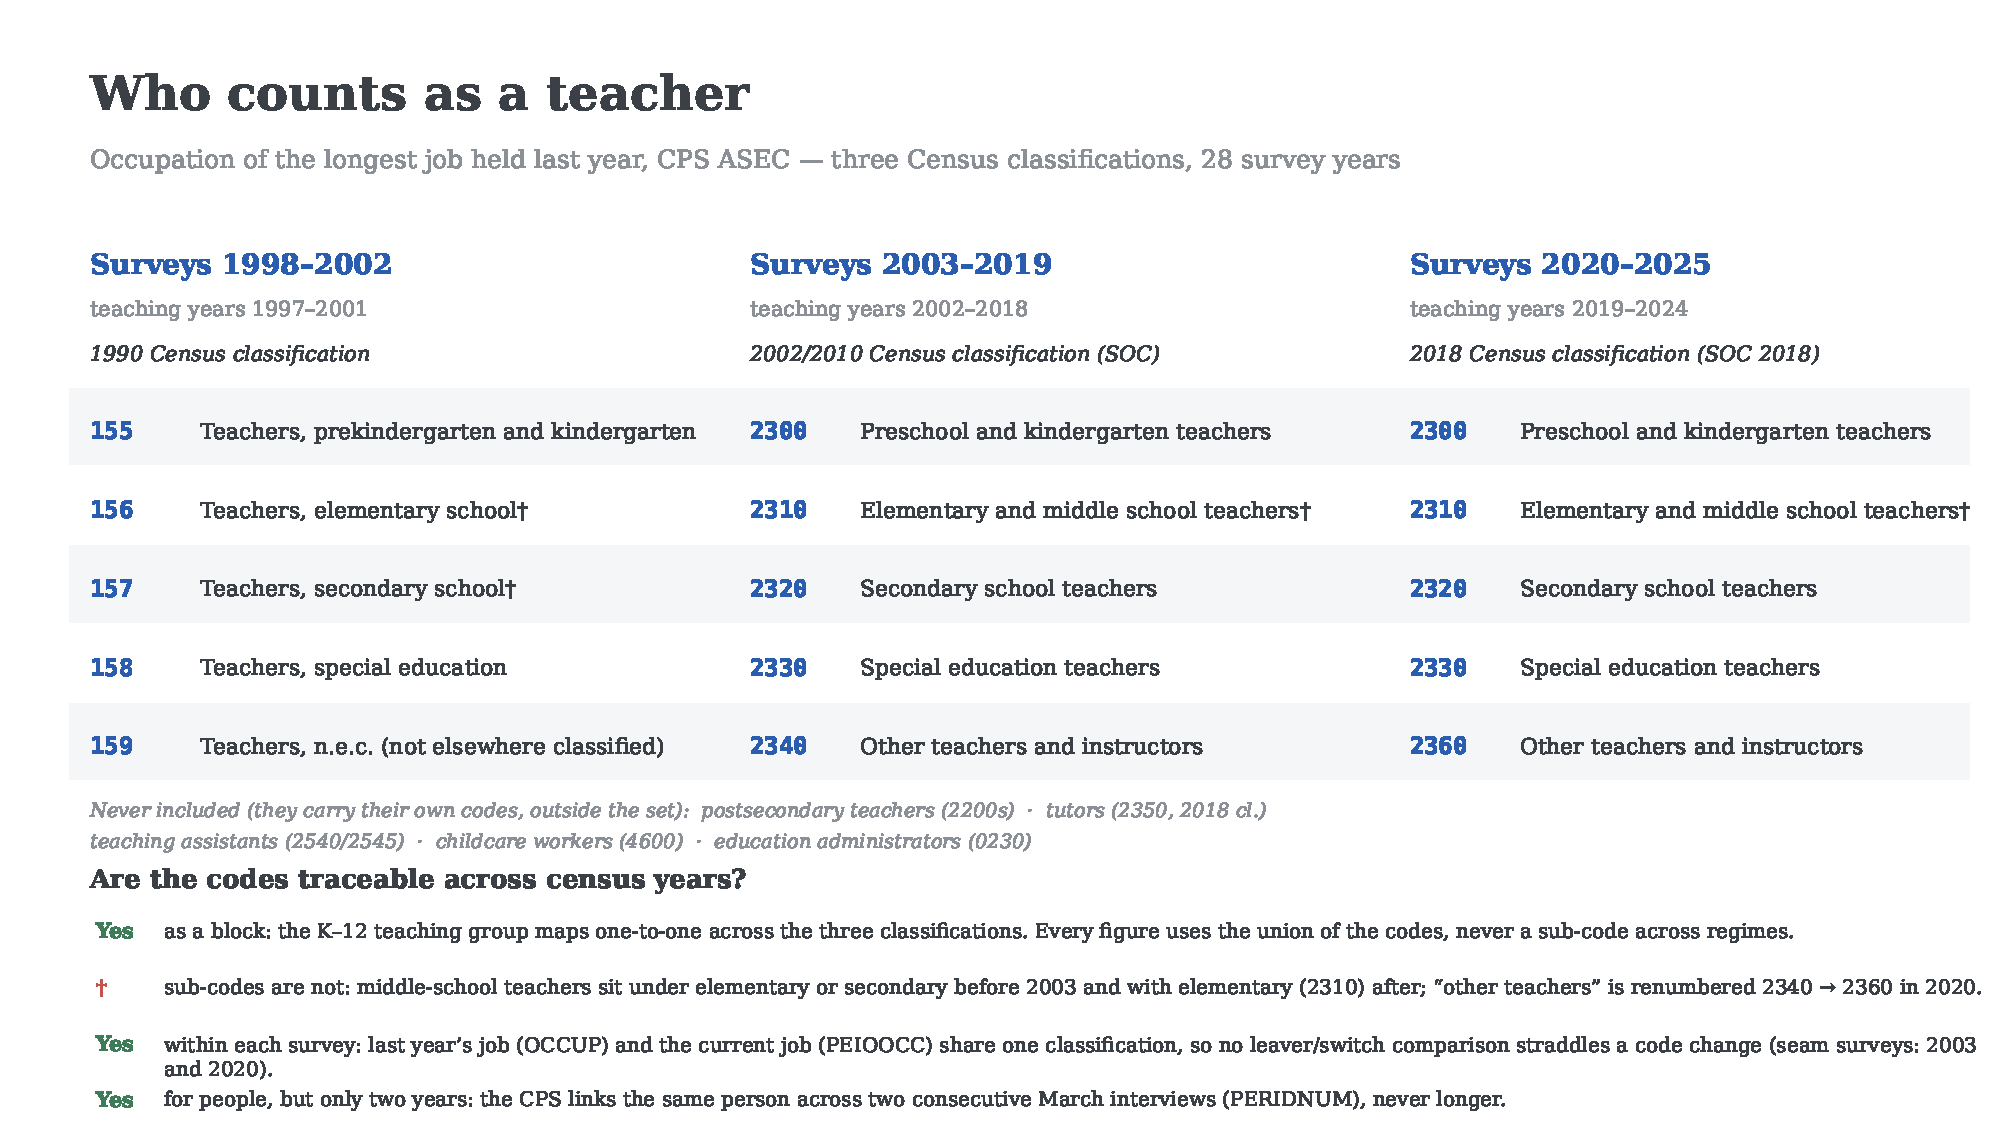
\includegraphics[width=0.98\textwidth]{figures/codes_slide.pdf}
  \end{center}
\end{frame}

% ================= D. Two ways to measure =================
\begin{frame}{Two ways to measure the leaving rate}
  \vspace{0.4em}
  \begin{columns}[T]
    \begin{column}{0.48\textwidth}
      \msg{Follow the person, year to year}\\[0.9em]
      {\small The rotation shows the same individual twelve months apart.
       The CPS has no person identifier, so records are linked on fields
       common to both years:}\\[0.7em]
      {\small
      \begin{tabular}{@{}l@{}}
        household identifier\\
        dwelling identifier\\
        person line number within the household\\[0.4em]
        \color{mut}validated on sex, race,\\
        \color{mut}and age advancing 0--2 years
      \end{tabular}}
    \end{column}
    \begin{column}{0.48\textwidth}
      \msg{Ask about last year, each March}\\[0.9em]
      {\small The supplement's retrospective question. Whoever reports
       teaching as last year's longest job, and no longer teaches at the
       March interview, left within the year.}\\[0.7em]
      {\small\color{mut} The measure used in the literature so far.}
    \end{column}
  \end{columns}
\end{frame}

% ================= E. Defining the leaver in the panel =================
\begin{frame}{Measuring the leaving rate: the alternatives, side by side}
  \begin{center}
  \footnotesize
  \begin{tabular}{p{2.3cm}p{3.3cm}p{4.1cm}p{3.2cm}}
    \toprule
    Measure & A teacher is\ldots & A leaver is\ldots & Rests on\ldots \\
    \midrule
    Annual recall &
      whoever taught as last year's longest job &
      no longer teaching at the March interview &
      accurate recall of the previous year \\[0.9em]
    Occupation pair &
      a teaching occupation code one year ago &
      a different occupation code today &
      a current code existing; fails for the non-employed \\[0.9em]
    \msg{Panel (benchmark)} &
      teaching in two or more year-1 interviews &
      never teaching in year 2, given two or more interviews, one outside
      the summer &
      correct linkage of persons across waves \\[0.9em]
    Month pairs, any sighting &
      every teaching month, or a single sighting &
      not teaching twelve months after each month &
      one person counting several times; admits one-month spells \\
    \bottomrule
  \end{tabular}
  \end{center}
  \vspace{0.3em}
  {\footnotesize\color{mut} Same records throughout; only the definition
   changes. Each row answers the same three questions.}
\end{frame}

\begin{frame}{One dataset, one rate per definition}
  \begin{center}
    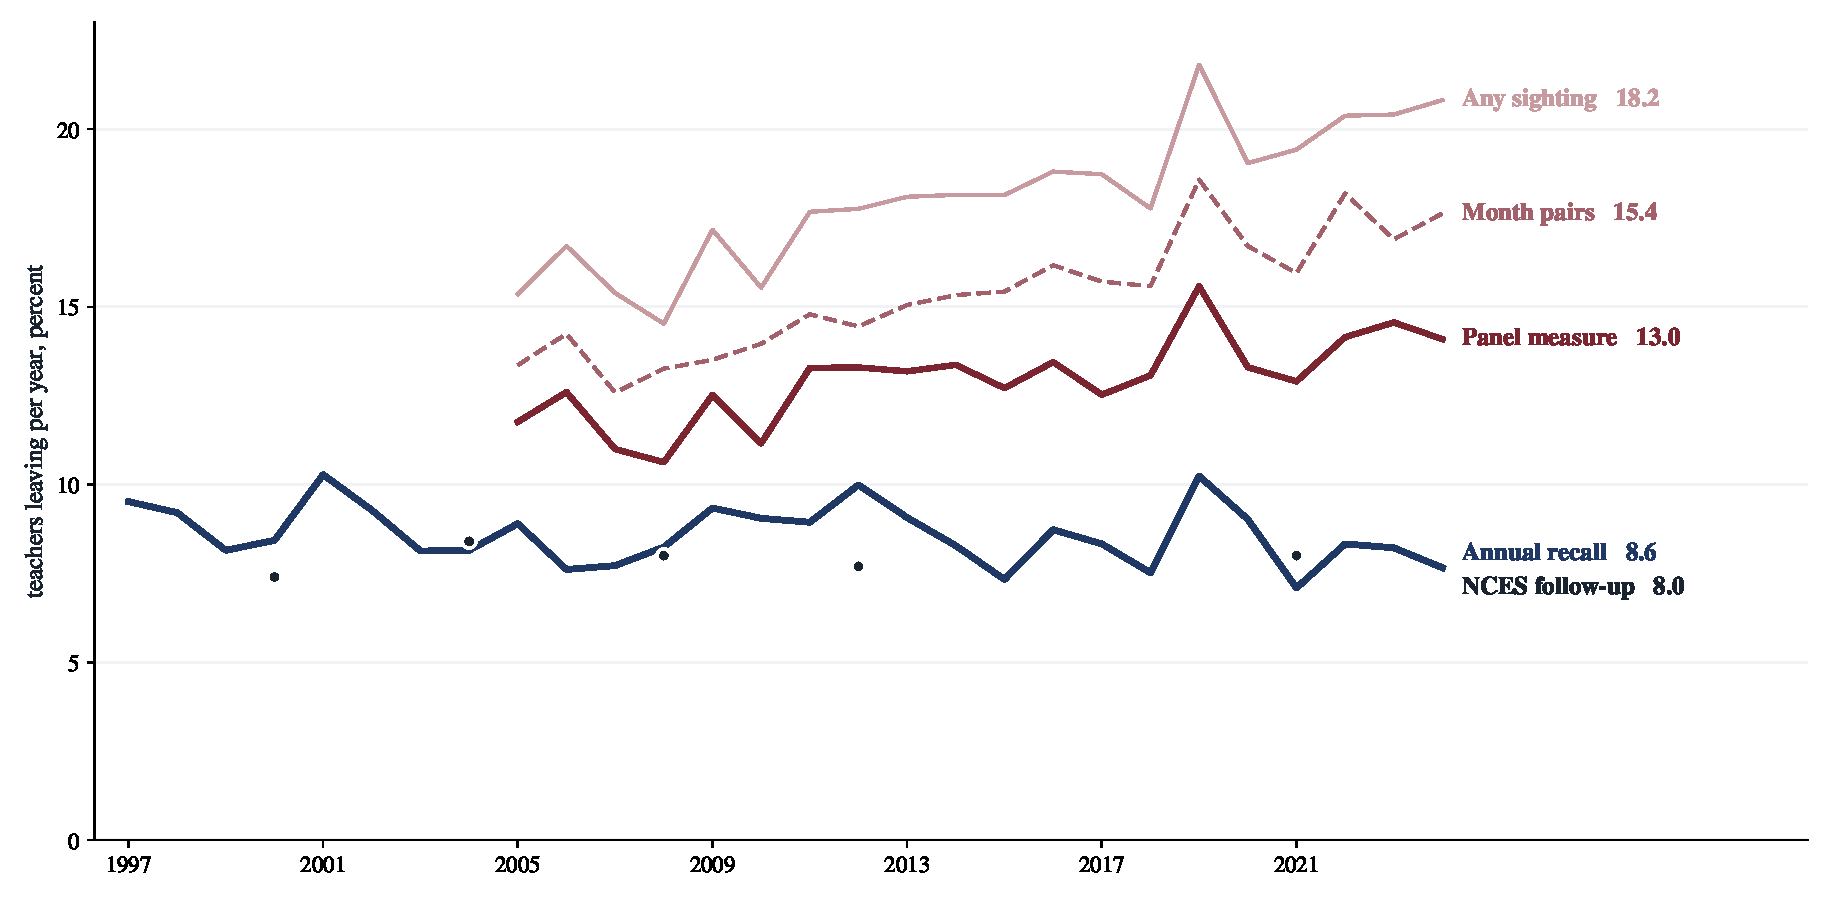
\includegraphics[width=0.92\textwidth]{figures/v_allseries.pdf}
  \end{center}
  \vspace{-0.4em}
  {\small \msg{Message.} The definition of a leaver moves the measured rate by a factor of nearly four.}\\[0.15em]
  {\small {\color{burg}\bfseries Policy.} Comparisons across studies and countries must hold the definition fixed.}
\end{frame}

% ================= F. Results =================
\begin{frame}{Why teachers leave: what the CPS can and cannot see}
  \begin{center}
  \begin{tabular}{ll}
    \toprule
    Reasons identified in the literature     & Observed in the CPS? \\
    \midrule
    Working conditions                       & \color{mut}no  \\
    Organizational support (mentoring, leadership) & \color{mut}no  \\
    Autonomy and intrinsic motives           & \color{mut}no  \\
    Financial factors                        & \color{navy}\textbf{yes} \\
    Personal life-cycle motives              & \color{navy}\textbf{yes} \\
    \midrule
    Sociodemographic characteristics         & \color{navy}\textbf{yes} \\
    \bottomrule
  \end{tabular}
  \end{center}
  \vspace{0.6em}
  {\footnotesize\color{mut} Five broad families of reasons from our review
   of the literature. The CPS covers the economic and life-cycle margins.}
\end{frame}

\begin{frame}{Five messages}
  \vspace{0.3em}
  \begin{enumerate}\setlength\itemsep{0.95em}
    \item Economic and employment conditions correlate with leaving far more
          than demographics.
    \item Exits concentrate where attachment and annual pay are lowest:
          part-time and part-year teachers in the bottom of the earnings
          distribution.
    \item Those same exits lead \emph{out of employment}, not to better-paid
          jobs: two thirds of bottom-quintile leavers exit the labor force.
          Low pay and non-employment destinations are one phenomenon, not two.
    \item Life-cycle events are the largest single trigger: childbirth raises
          a woman's exit probability by about six points, more than in
          comparable professions.
    \item Pension coverage retains, and attrition differs widely across
          states: the actionable margins are contractual and institutional.
  \end{enumerate}
\end{frame}

\begin{frame}{Leaving teaching, 1997--2024}
  \begin{center}
    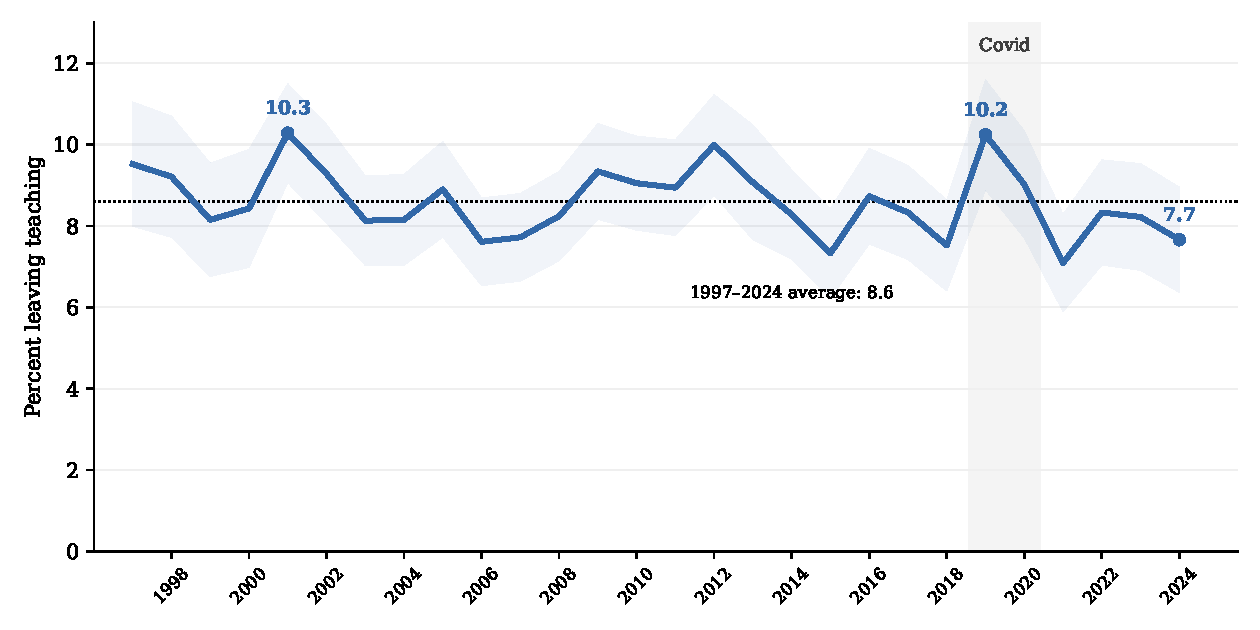
\includegraphics[height=0.66\textheight]{figures/g2_evolution.pdf}
  \end{center}
  \vspace{-0.3em}
  {\small \msg{Message.} The rate fluctuates around 8.6 percent with no trend: a persistent outflow, not a mounting exodus.}\\[0.15em]
  {\small {\color{burg}\bfseries Policy.} Retention faces a steady-state cost, not an emergency spike.}
\end{frame}

\begin{frame}{Leaving teaching, by school sector}
  \begin{center}
    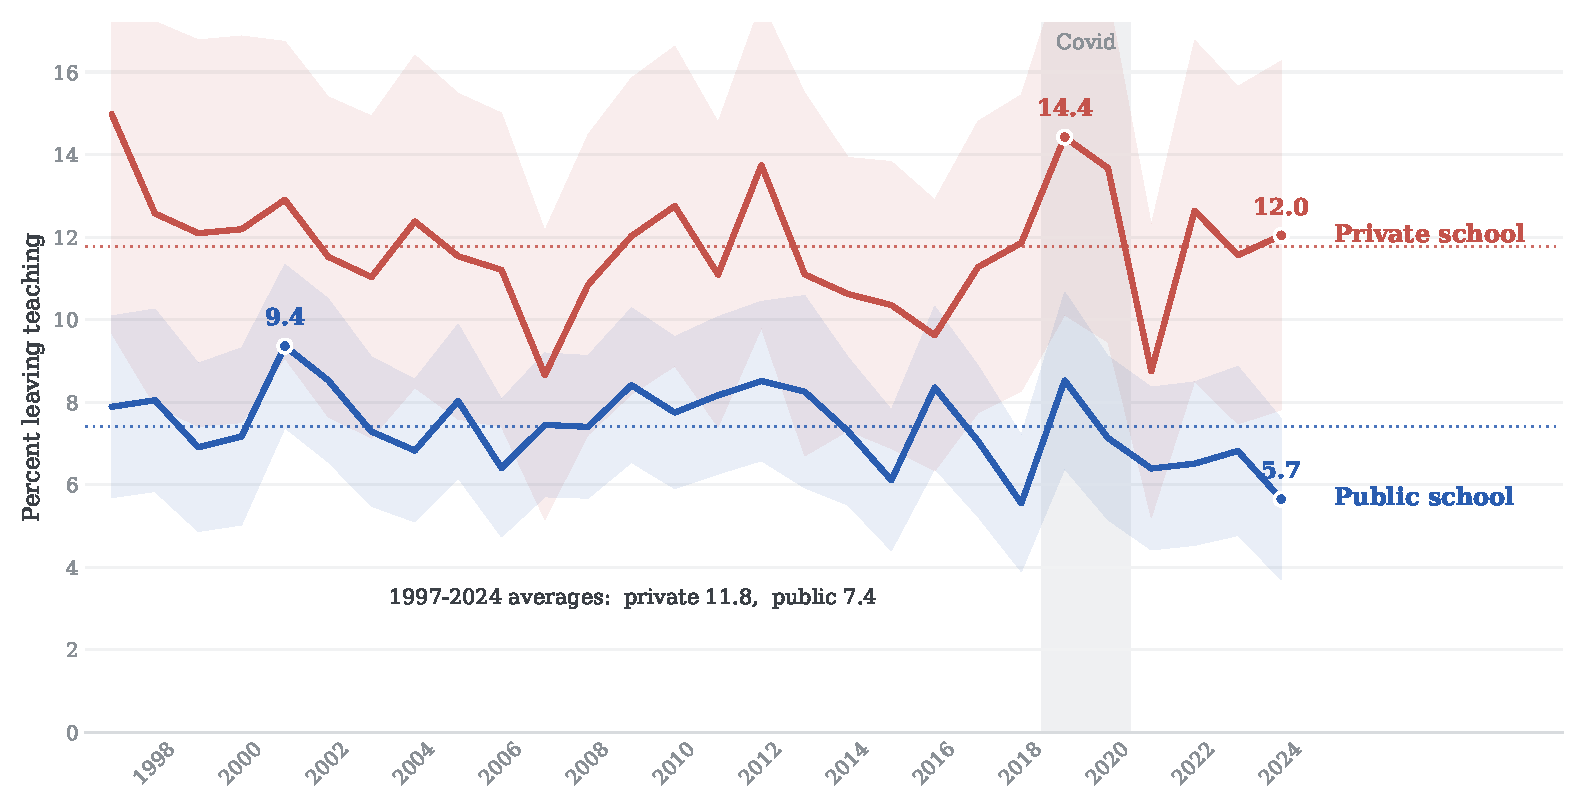
\includegraphics[height=0.66\textheight]{figures/pubpriv_series.pdf}
  \end{center}
  \vspace{-0.3em}
  {\small \msg{Message.} Private schools lose teachers at roughly twice the public rate.}\\[0.15em]
  {\small {\color{burg}\bfseries Policy.} Retention tracks contract structure, pay and pensions, not classroom conditions alone.}
\end{frame}

\begin{frame}{Leaving the occupation, by profession}
  \begin{center}
    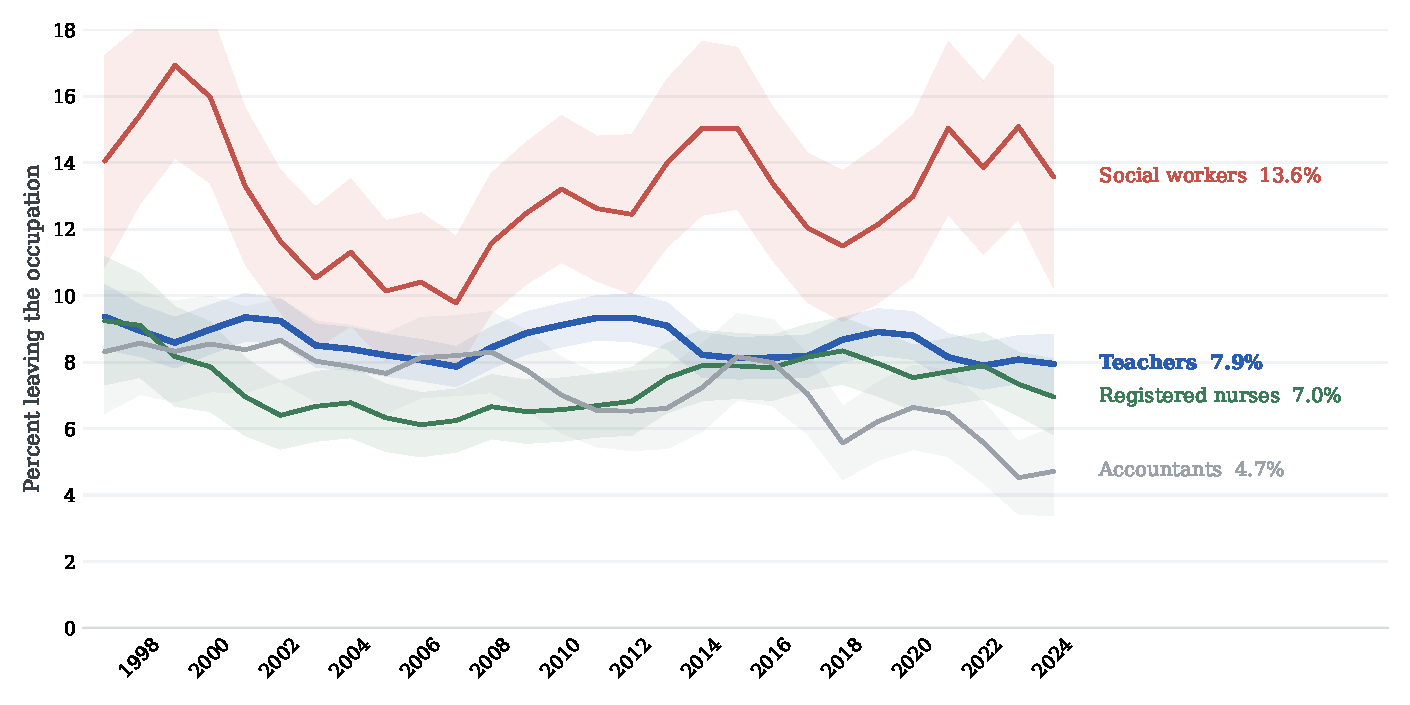
\includegraphics[height=0.66\textheight]{figures/leave_professions_deck.pdf}
  \end{center}
  \vspace{-0.3em}
  {\small \msg{Message.} Teacher attrition is unexceptional next to comparable professions: above nurses and accountants, well below social workers.}\\[0.15em]
  {\small {\color{burg}\bfseries Policy.} Benchmarks from other professions discipline how alarming any teacher figure should be.}
\end{frame}

\begin{frame}{Labor force exit of women, by profession}
  \begin{center}
    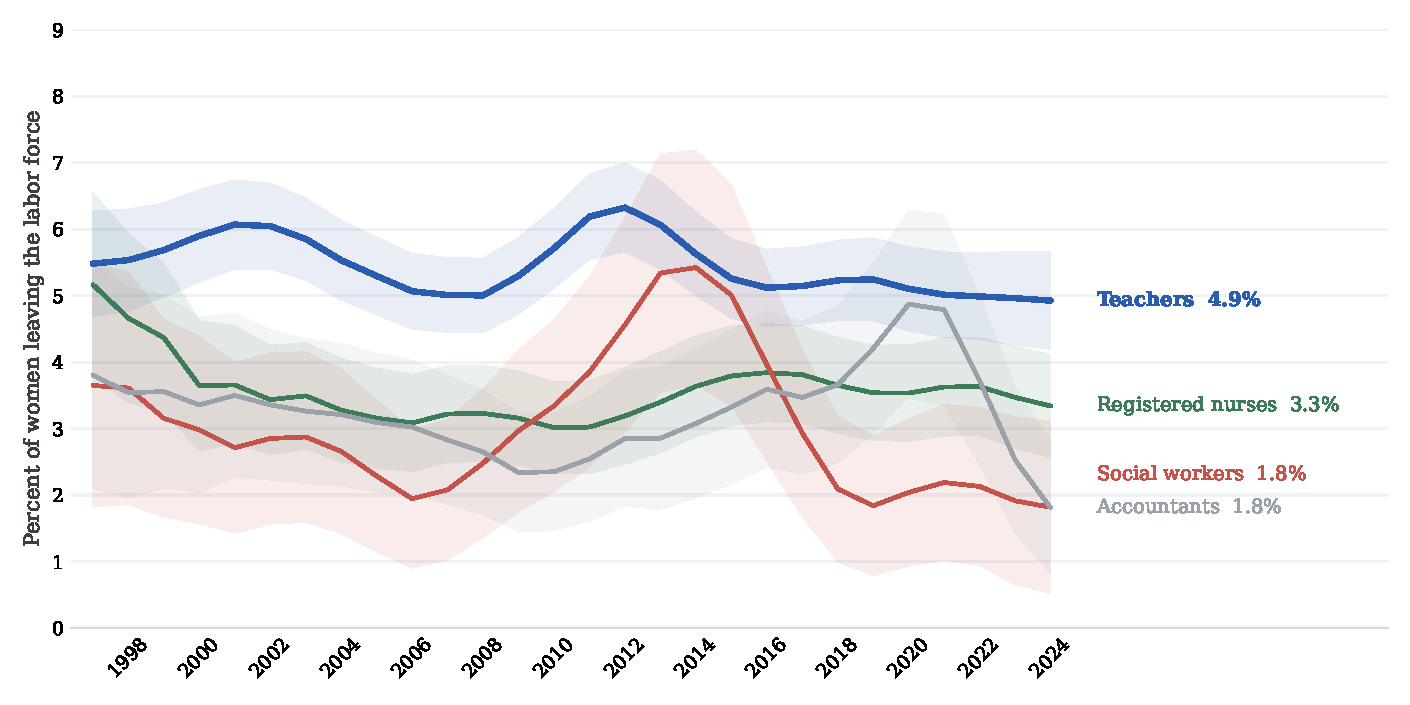
\includegraphics[height=0.66\textheight]{figures/lf_professions_deck.pdf}
  \end{center}
  \vspace{-0.3em}
  {\small \msg{Message.} Women teachers exit the labor force at about five percent a year, well above nurses, social workers and accountants.}\\[0.15em]
  {\small {\color{burg}\bfseries Policy.} The family-compatibility margin is specific to teaching, not to professional work in general.}
\end{frame}

\begin{frame}{Teachers leaving per year, across countries}
  \begin{center}
    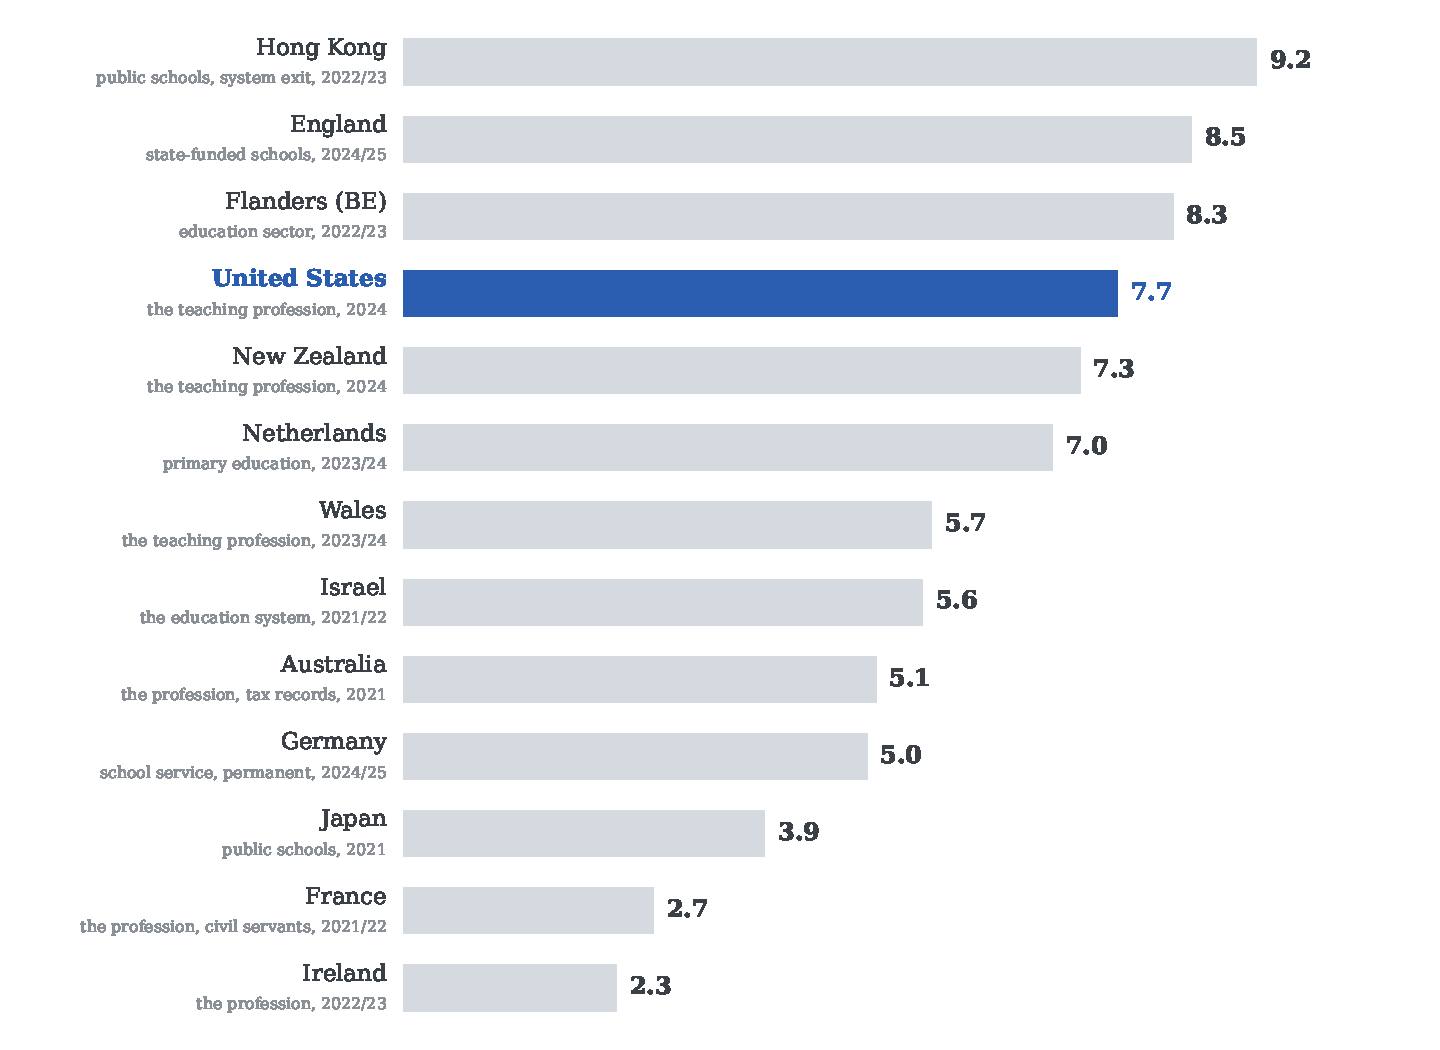
\includegraphics[height=0.62\textheight]{figures/intl_bars_deck.pdf}
  \end{center}
  \vspace{-0.3em}
  {\small \msg{Message.} The US sits in the upper range of the school systems that publish a rate.}\\[0.15em]
  {\small {\color{burg}\bfseries Policy.} Comparable, survey-based measurement is what makes this ranking possible.}
\end{frame}

\begin{frame}{Destinations of teachers who leave, 2024}
  \begin{center}
    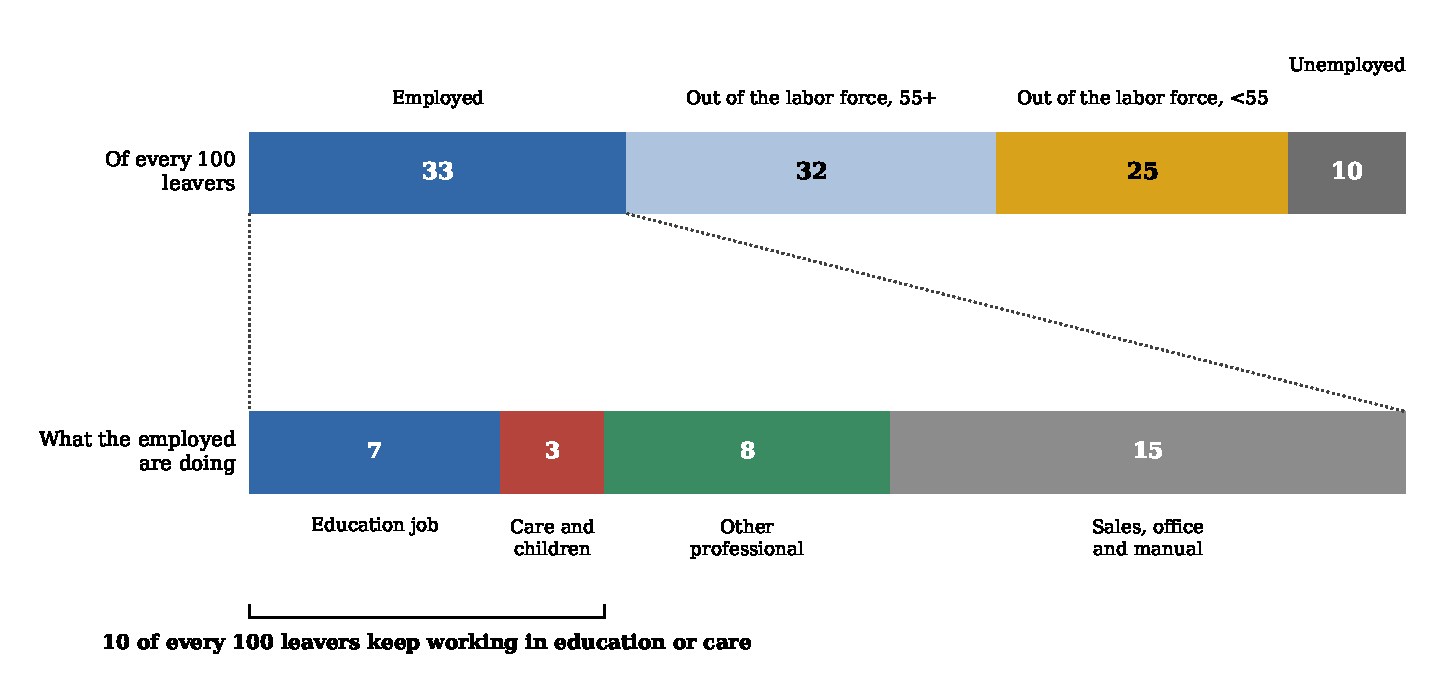
\includegraphics[height=0.66\textheight]{figures/g3_flow100_2024.pdf}
  \end{center}
  \vspace{-0.3em}
  {\small \msg{Message.} Of every hundred leavers, about a third take another job; most exit employment altogether.}\\[0.15em]
  {\small {\color{burg}\bfseries Policy.} Competing employers are not the main counterfactual; retirement and care are.}
\end{frame}

\begin{frame}{The routes out of teaching, 2002--2024}
  \begin{center}
    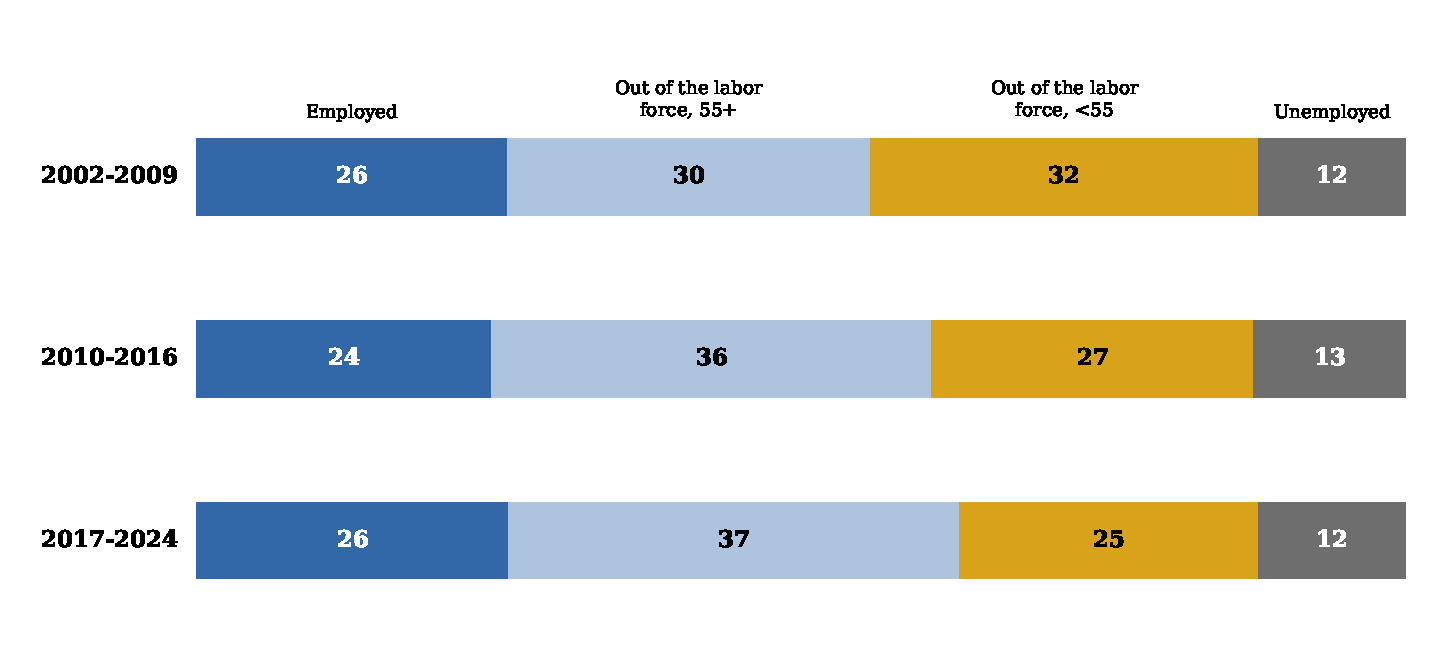
\includegraphics[height=0.66\textheight]{figures/routes_bars3.pdf}
  \end{center}
  \vspace{-0.3em}
  {\small \msg{Message.} The destination mix has been essentially stable for two decades.}\\[0.15em]
  {\small {\color{burg}\bfseries Policy.} The composition of the outflow is structural, not cyclical noise.}
\end{frame}

\begin{frame}{Who leaves the labor force before 55}
  \begin{center}
    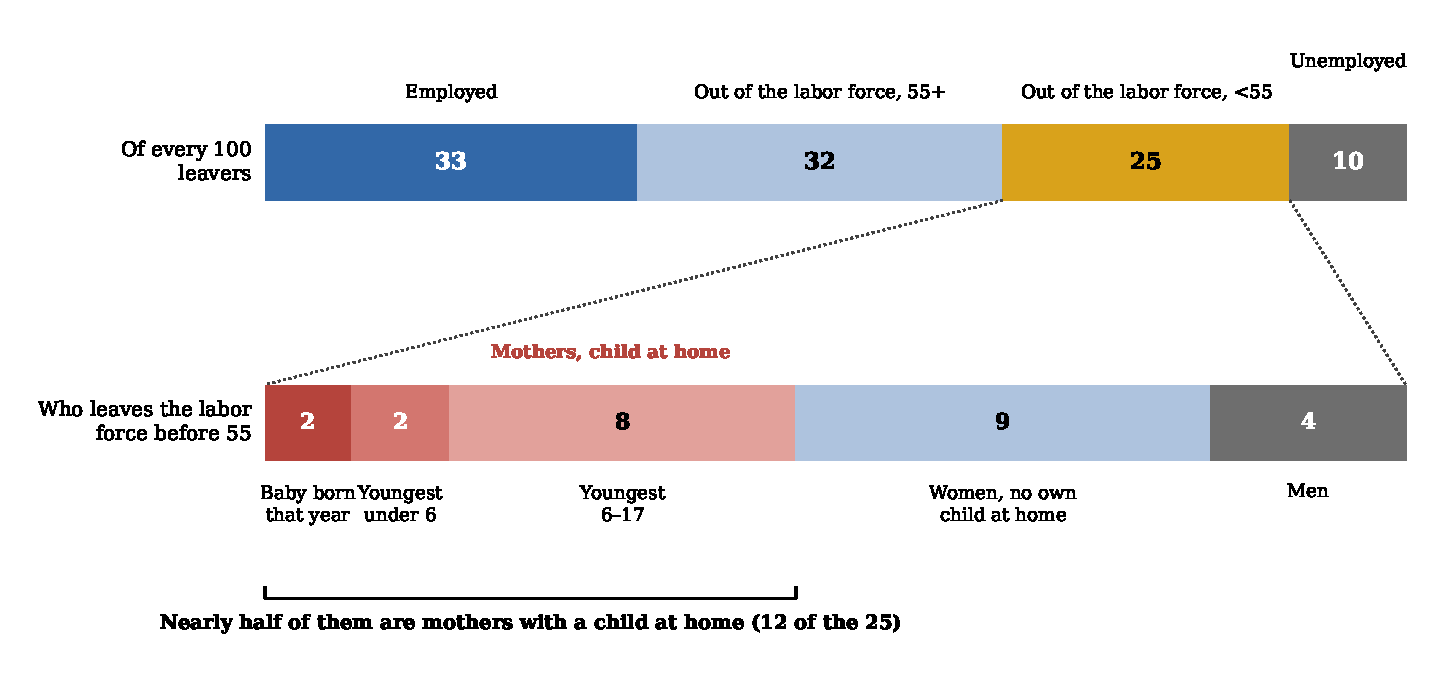
\includegraphics[height=0.66\textheight]{figures/yellow_flow2024.pdf}
  \end{center}
  \vspace{-0.3em}
  {\small \msg{Message.} Nearly half of the pre-55 labor-force exits are mothers with a child at home.}\\[0.15em]
  {\small {\color{burg}\bfseries Policy.} Childcare and parental-leave policy are retention policy.}
\end{frame}

\begin{frame}{Where the employed leavers go: every occupation}
  \begin{center}
    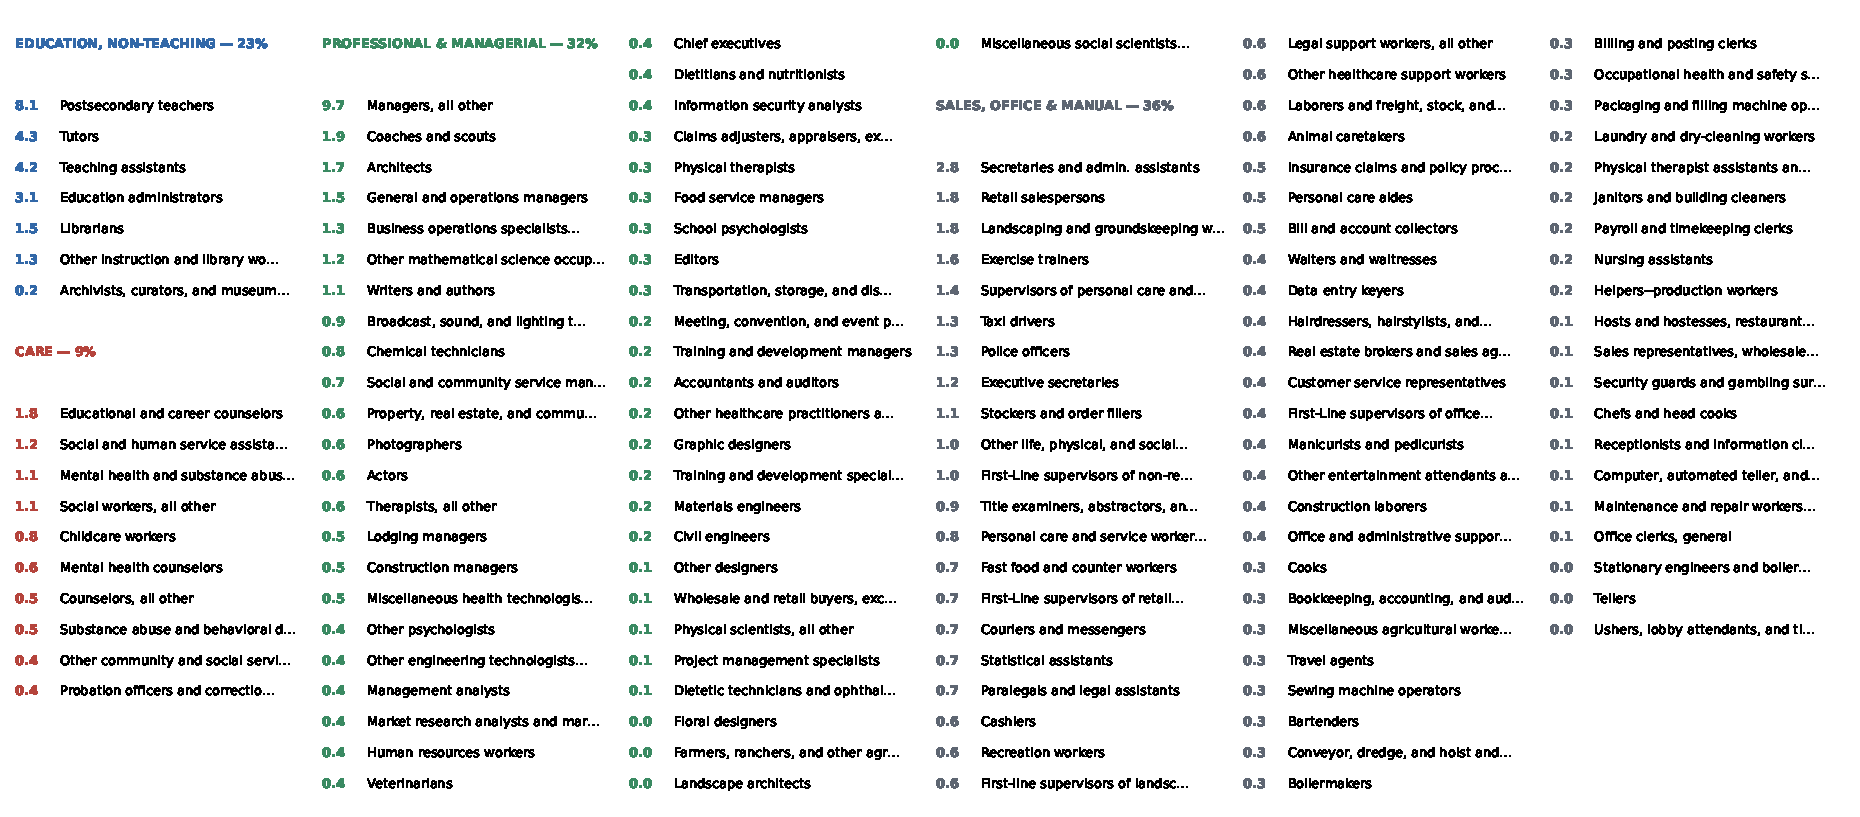
\includegraphics[height=0.66\textheight]{figures/occ_all_slide.pdf}
  \end{center}
  \vspace{-0.3em}
  {\small \msg{Message.} Employed leavers scatter widely; the largest block stays in education outside the classroom.}\\[0.15em]
  {\small {\color{burg}\bfseries Policy.} Skills remain in the education orbit, so re-entry is a realistic margin.}
\end{frame}

\begin{frame}{Leaving teaching, by age and route}
  \begin{center}
    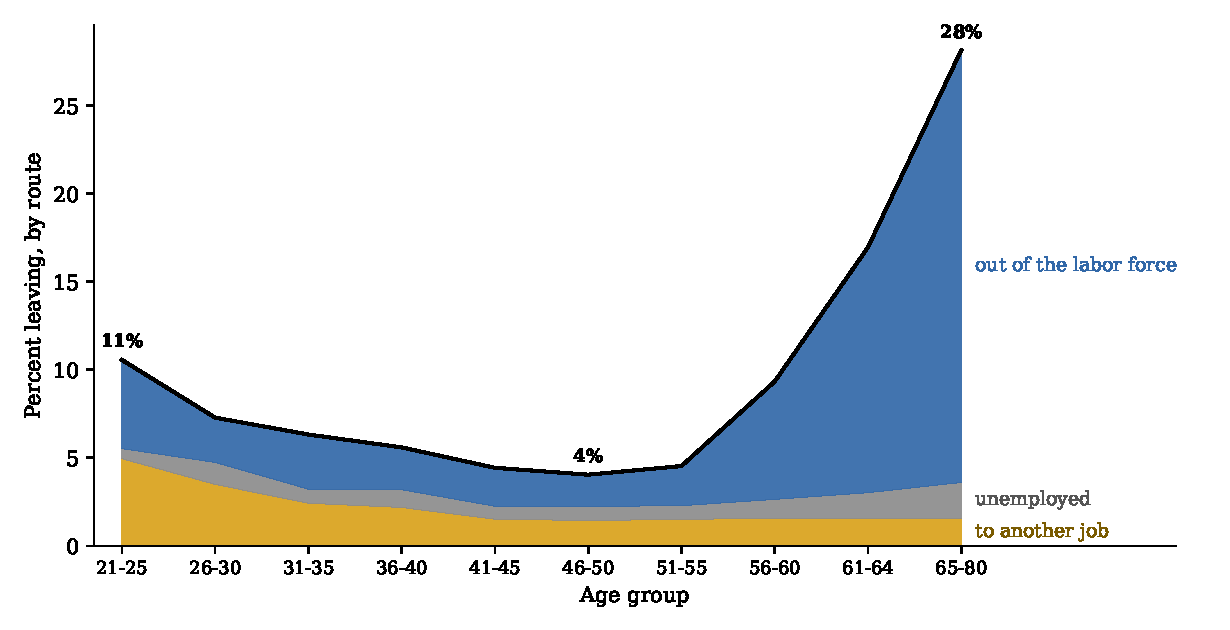
\includegraphics[height=0.66\textheight]{figures/g4_routes_age.pdf}
  \end{center}
  \vspace{-0.3em}
  {\small \msg{Message.} Leaving is U-shaped in age, and non-employment dominates both ends of the career.}\\[0.15em]
  {\small {\color{burg}\bfseries Policy.} Early-career and pre-retirement exits call for different instruments.}
\end{frame}

\begin{frame}{The econometric specification}
  \vspace{0.2em}
  \[
    \Pr\bigl(\text{Leave}_{it}=1 \mid x_{it}\bigr)
    \;=\;
    \Phi\Bigl(
      \underbrace{\text{attach}_{it}'\beta_1}_{\substack{\text{full year,}\\ \text{part-time}}}
      +\underbrace{\text{comp}_{it}'\beta_2}_{\substack{\text{pension,}\\ \text{public school}}}
      +\underbrace{\text{fam}_{it}'\beta_3}_{\substack{\text{new baby, children,}\\ \text{marital status}}}
      +\underbrace{\text{dem}_{it}'\beta_4}_{\substack{\text{age, age}^2\text{, sex,}\\ \text{race, education}}}
      +\;\delta_t
    \Bigr)
  \]
  \vspace{0.4em}
  \begin{itemize}\setlength\itemsep{0.5em}
    \item {\small Probit on college-graduate teachers, pooled 2015--2024,
          with calendar-year effects $\delta_t$; $n=28{,}900$.}
    \item {\small Average marginal effects reported, in percentage points.}
    \item {\small Robust to logit and weighted LPM, state and year fixed
          effects, the full 1997--2024 window ($n=85{,}430$), and the
          occupation-pair definition of leaving.}
  \end{itemize}
\end{frame}

\begin{frame}{Average marginal effects on the probability of leaving}
  \begin{center}
    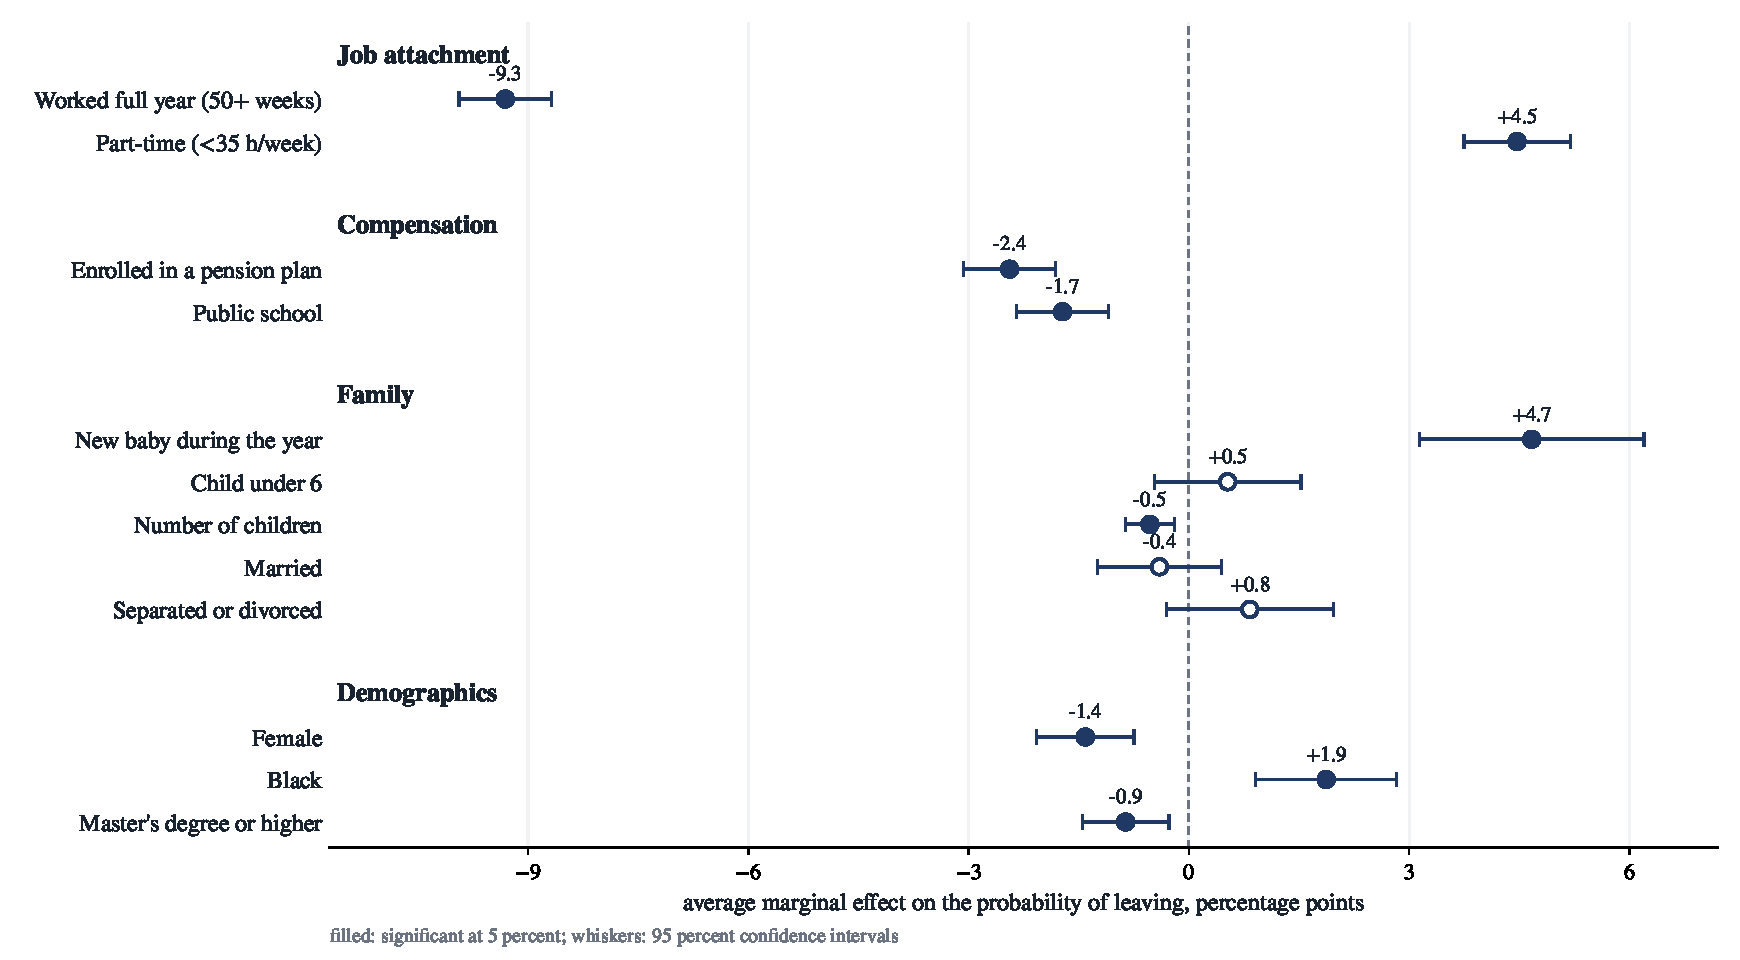
\includegraphics[height=0.66\textheight]{figures/ame_seminar.pdf}
  \end{center}
  \vspace{-0.3em}
  {\small \msg{Message.} Job attachment and compensation dominate; demographic differences are small.}\\[0.15em]
  {\small {\color{burg}\bfseries Policy.} The actionable levers are contractual: full-year contracts, pension coverage.}
\end{frame}

\begin{frame}{The age profile of leaving, by route}
  \begin{center}
    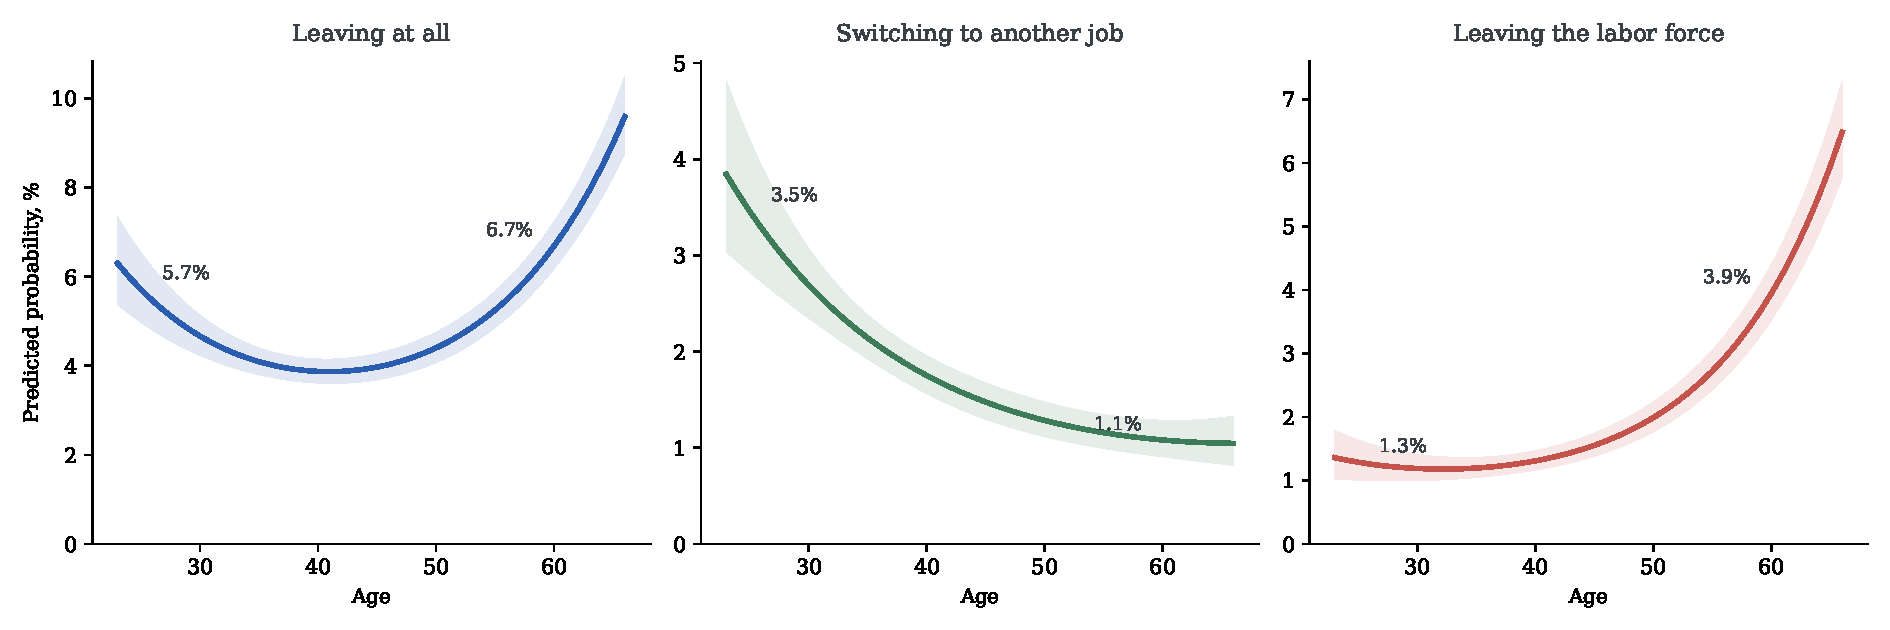
\includegraphics[height=0.66\textheight]{figures/u_routes_deck.pdf}
  \end{center}
  \vspace{-0.3em}
  {\small \msg{Message.} Young teachers switch to other jobs; older teachers leave the labor force.}\\[0.15em]
  {\small {\color{burg}\bfseries Policy.} The two peaks of the U respond to different policies.}
\end{frame}

\begin{frame}{The effect of a new baby, by profession}
  \begin{center}
    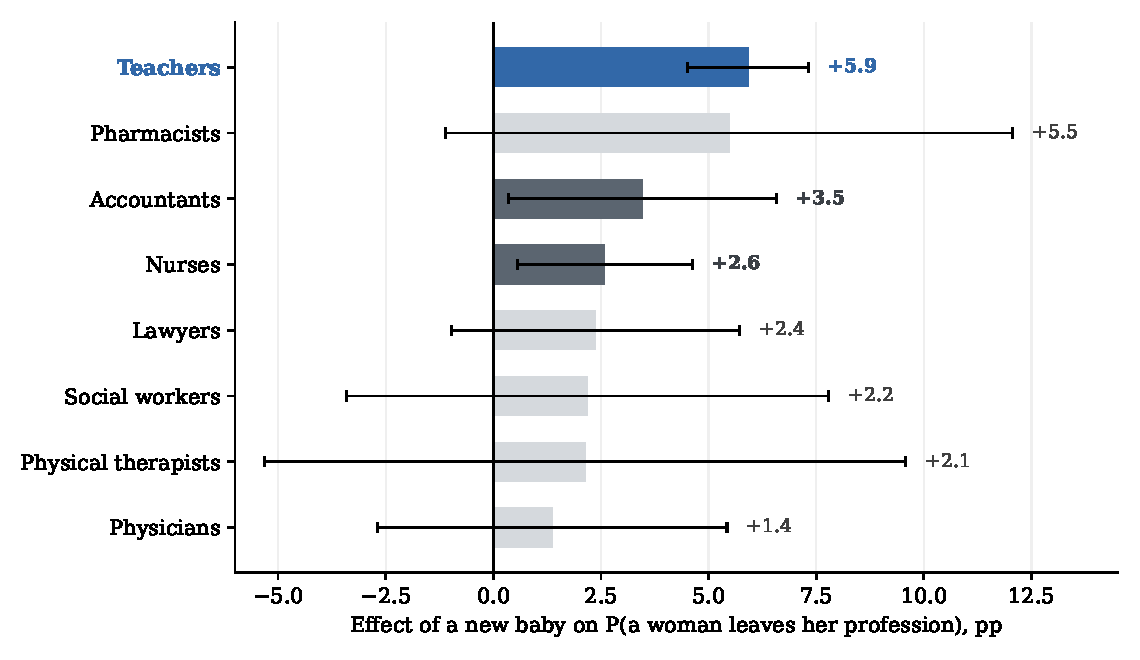
\includegraphics[height=0.66\textheight]{figures/g8_newbaby.pdf}
  \end{center}
  \vspace{-0.3em}
  {\small \msg{Message.} A new baby raises a woman teacher's exit probability by 5.9 points, the largest effect among comparable professions.}\\[0.15em]
  {\small {\color{burg}\bfseries Policy.} Parental leave and childcare support target the largest single observable trigger.}
\end{frame}

\begin{frame}{Leaving teaching and the unemployment rate}
  \begin{center}
    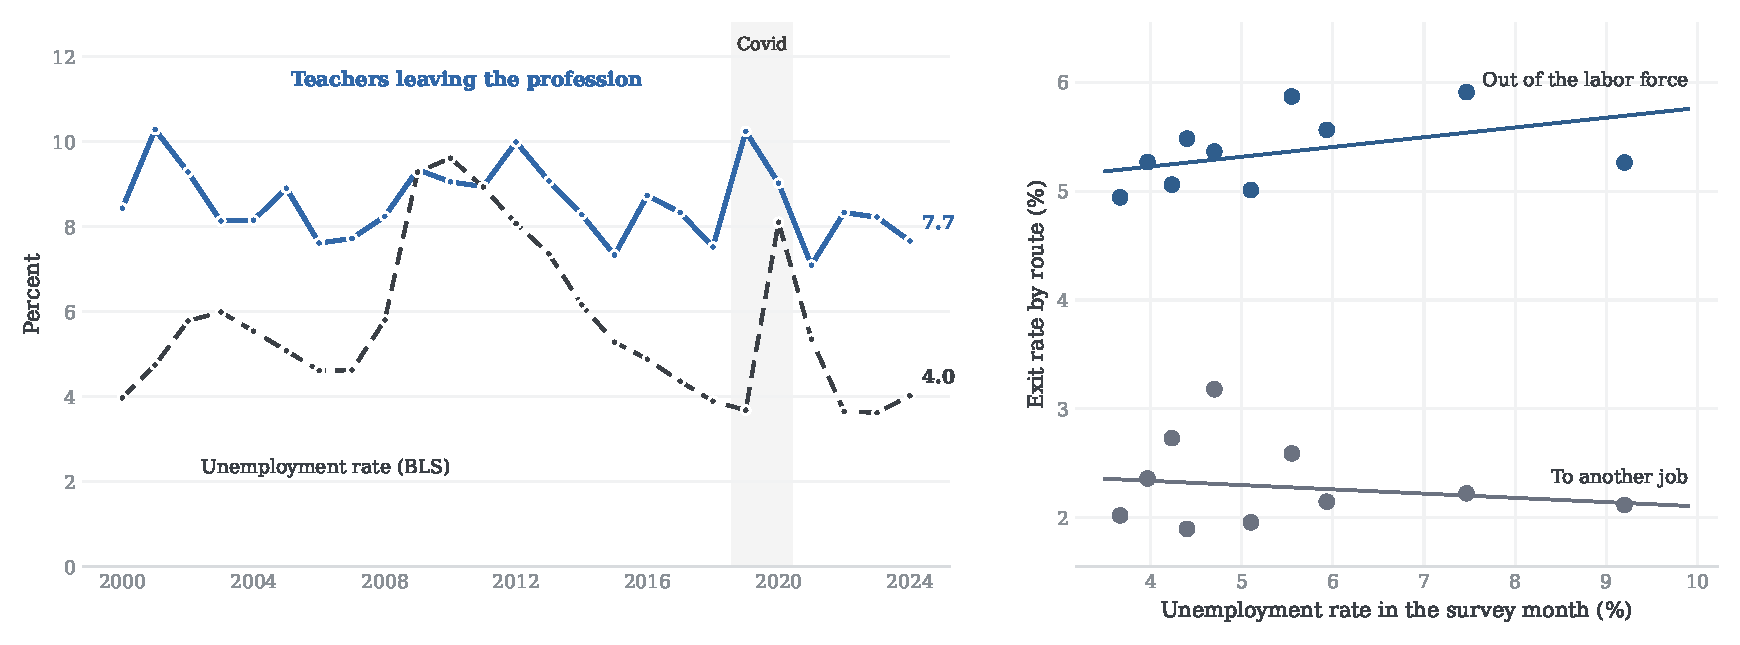
\includegraphics[height=0.66\textheight]{figures/n5_cyclicality.pdf}
  \end{center}
  \vspace{-0.3em}
  {\small \msg{Message.} Exits into non-employment rise with unemployment; job-to-job exits do not.}\\[0.15em]
  {\small {\color{burg}\bfseries Policy.} Downturns intensify the non-employment route; support should be countercyclical.}
\end{frame}

\begin{frame}{State-level cyclicality of leaving}
  \begin{center}
    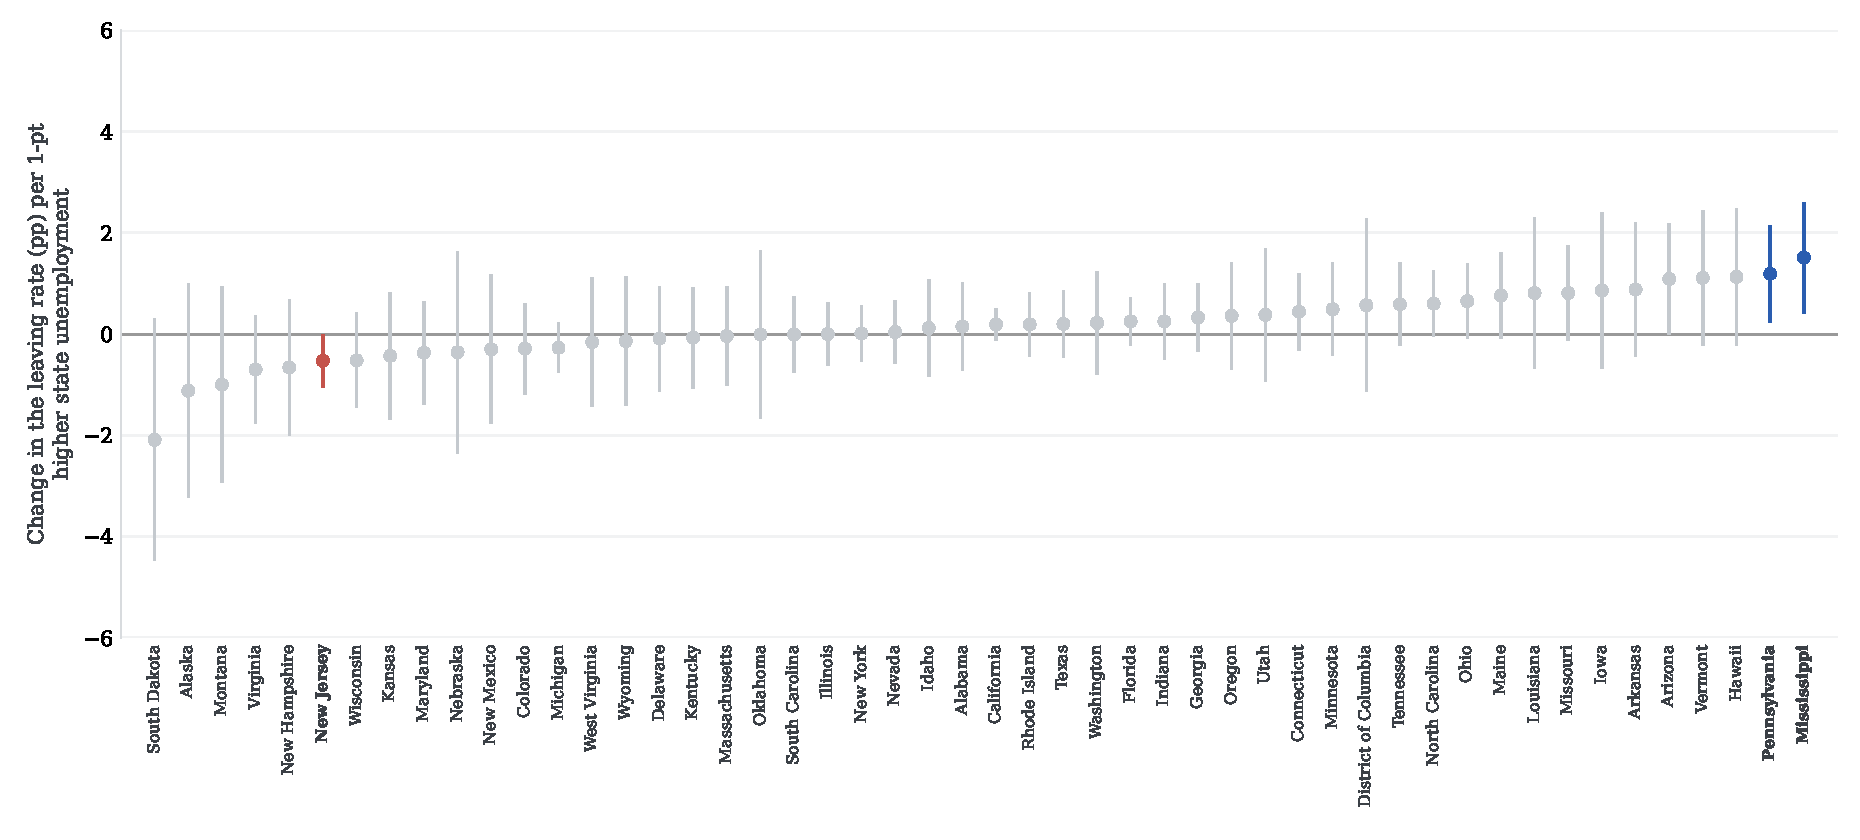
\includegraphics[height=0.66\textheight]{figures/states_landscape.pdf}
  \end{center}
  \vspace{-0.3em}
  {\small \msg{Message.} States differ in how strongly teacher exits respond to the local cycle.}\\[0.15em]
  {\small {\color{burg}\bfseries Policy.} National averages hide state-level exposure to downturns.}
\end{frame}

\begin{frame}{Attrition levels across states}
  \begin{center}
    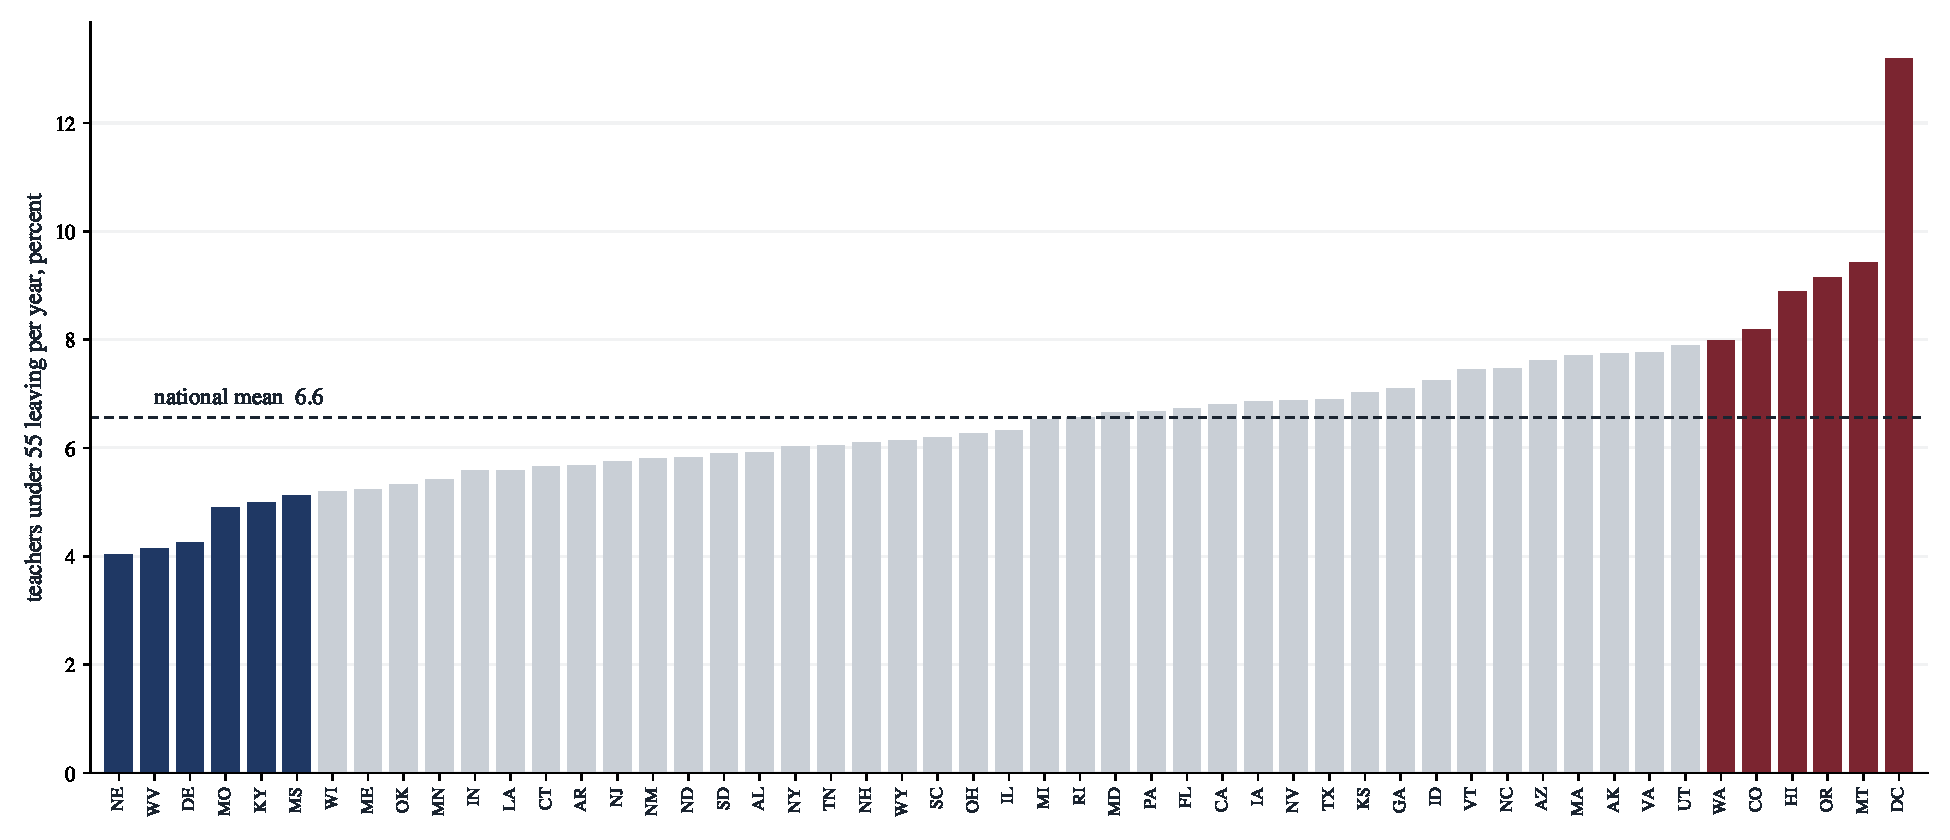
\includegraphics[height=0.66\textheight]{figures/states_level.pdf}
  \end{center}
  \vspace{-0.3em}
  {\small \msg{Message.} Mean attrition of teachers under 55 ranges from about 4 to 13 percent across jurisdictions.}\\[0.15em]
  {\small {\color{burg}\bfseries Policy.} State pay scales, pensions and institutions are first-order.}
\end{frame}

\begin{frame}{Real earnings growth by profession since 1997}
  \begin{center}
    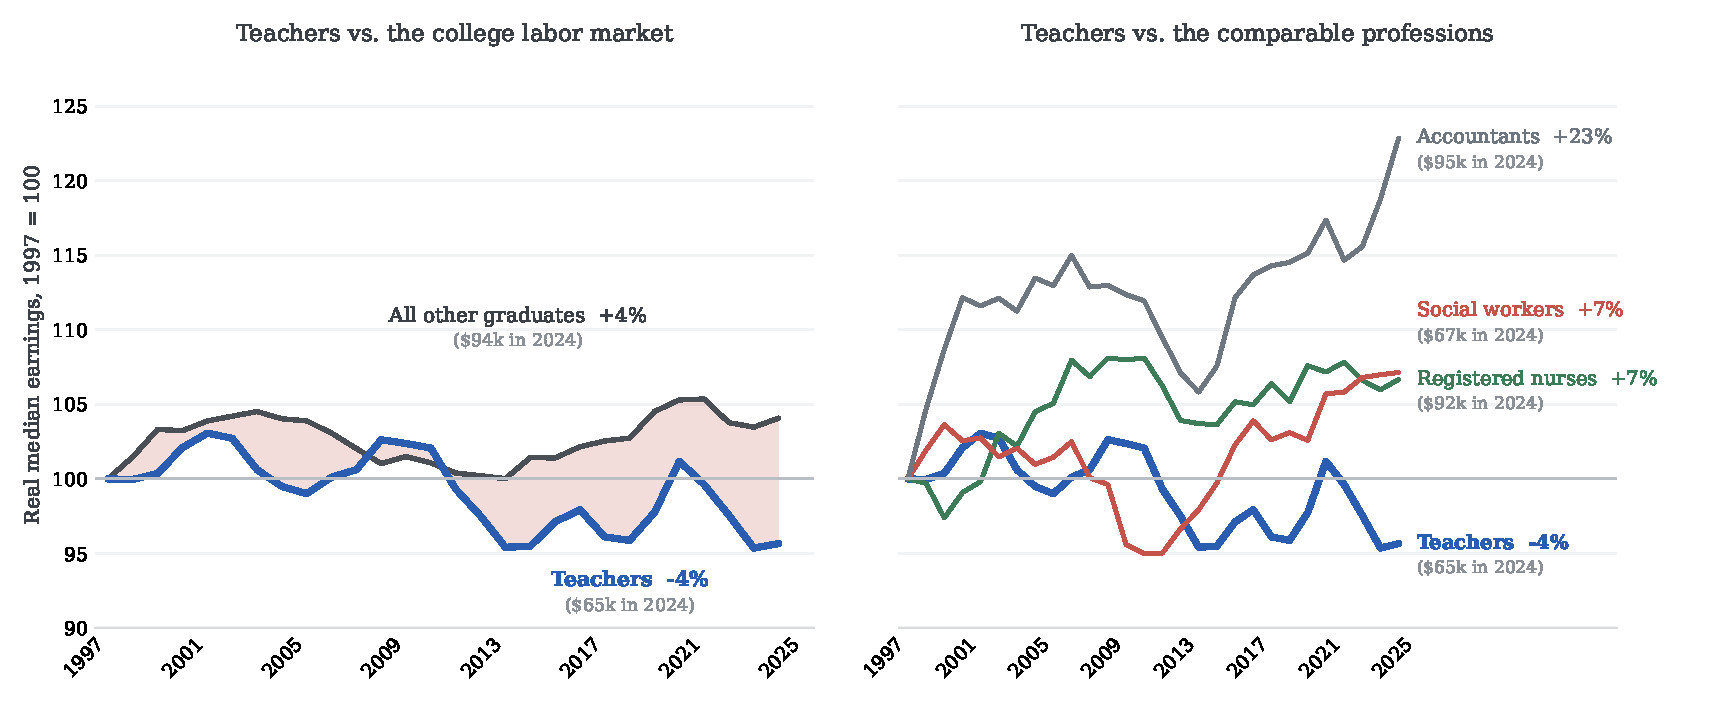
\includegraphics[height=0.66\textheight]{figures/msgA3.pdf}
  \end{center}
  \vspace{-0.3em}
  {\small \msg{Message.} Teachers' real median earnings fell 4 percent since 1997 while other graduates gained.}\\[0.15em]
  {\small {\color{burg}\bfseries Policy.} The relative-pay gap compounds slowly; it is a stock, not a shock.}
\end{frame}

\begin{frame}{Leaving, by position in the teacher pay distribution}
  \begin{center}
    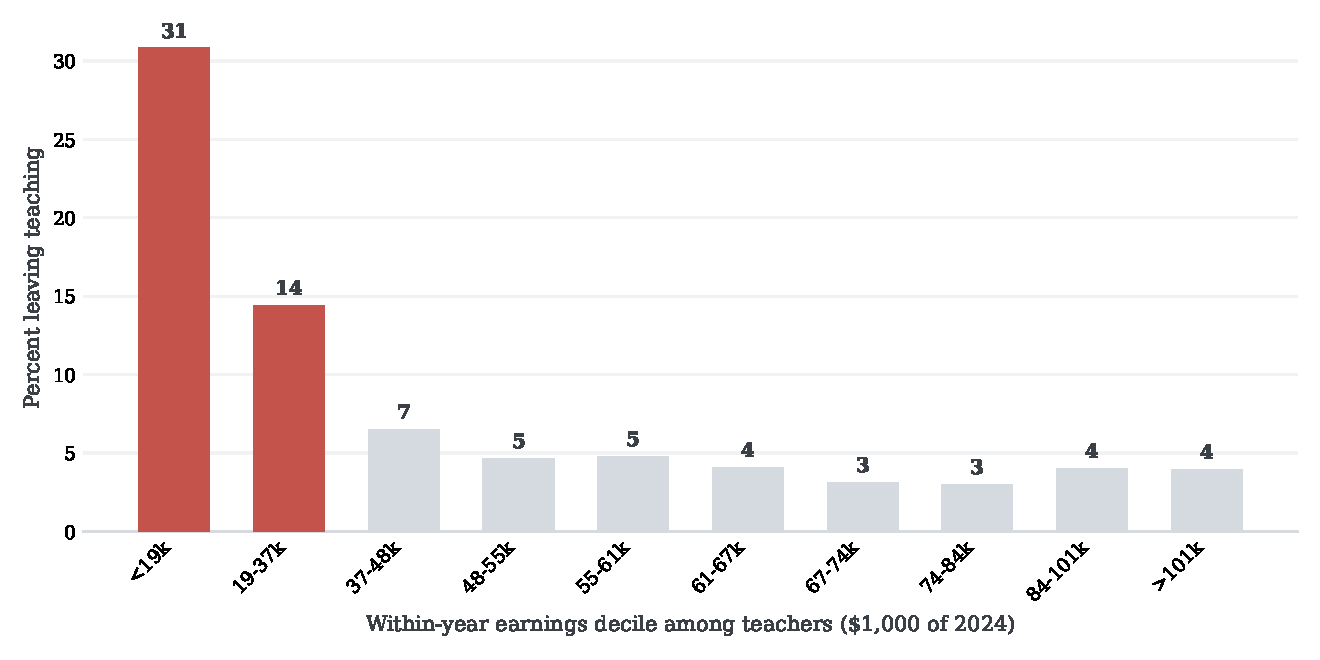
\includegraphics[height=0.66\textheight]{figures/pay3_deciles_deck.pdf}
  \end{center}
  \vspace{-0.3em}
  {\small \msg{Message.} Leaving concentrates sharply in the lowest earnings deciles, mostly part-year teachers.}\\[0.15em]
  {\small {\color{burg}\bfseries Policy.} Stabilizing the bottom of the distribution buys the most retention.}
\end{frame}

\begin{frame}{Pay compression: teachers and comparable professions}
  \begin{center}
    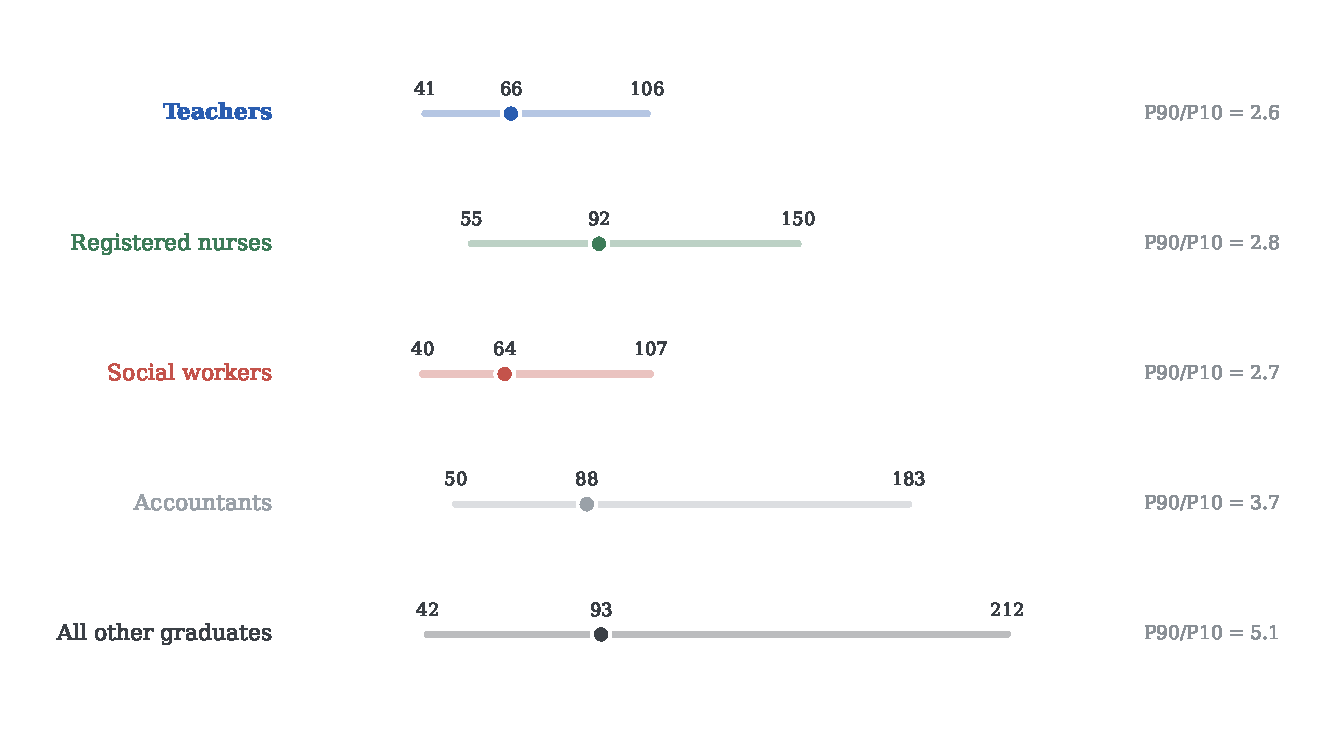
\includegraphics[height=0.66\textheight]{figures/pay5_compression_deck.pdf}
  \end{center}
  \vspace{-0.3em}
  {\small \msg{Message.} Teacher pay is compressed: a 90/10 ratio of 2.6 against 5.1 for all other graduates.}\\[0.15em]
  {\small {\color{burg}\bfseries Policy.} Staying offers little earnings upside; career ladders would widen the right tail.}
\end{frame}

\begin{frame}{The earnings change of leaving, by destination}
  \begin{center}
    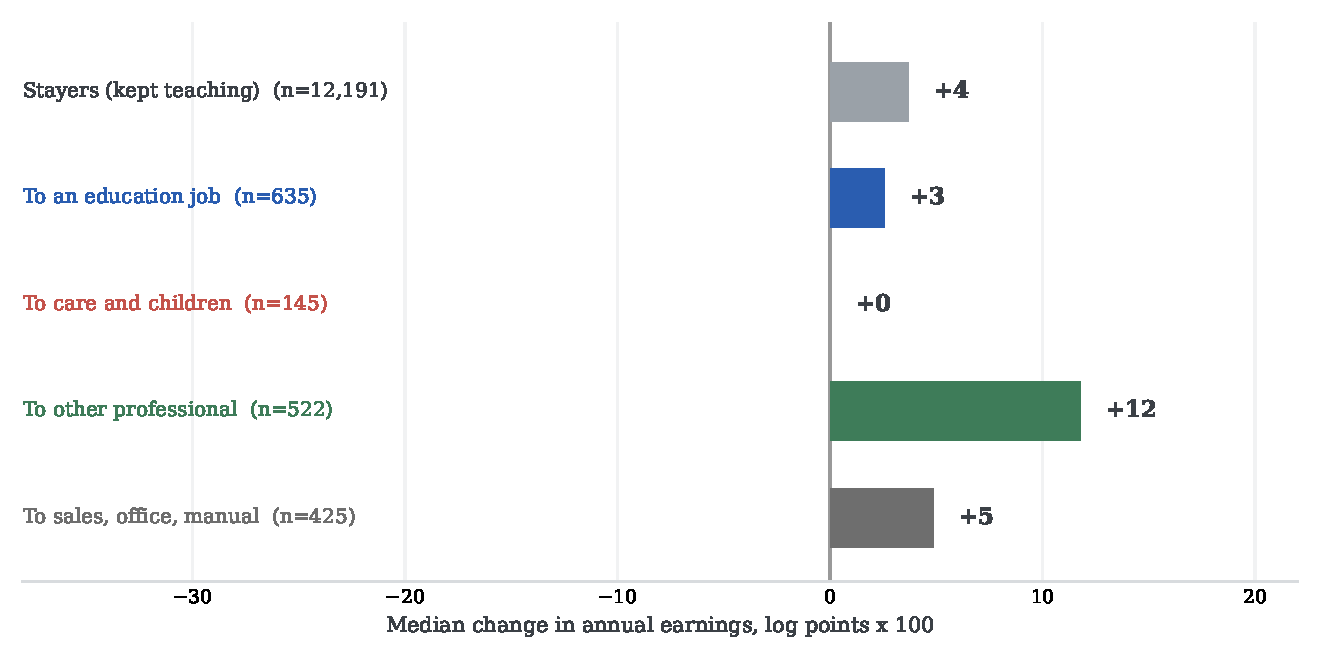
\includegraphics[height=0.66\textheight]{figures/pay7_destinations_deck.pdf}
  \end{center}
  \vspace{-0.3em}
  {\small \msg{Message.} Leavers who move to other professional jobs gain about 12 log points; moves near education gain little.}\\[0.15em]
  {\small {\color{burg}\bfseries Policy.} The outside option is real for those able to take it.}
\end{frame}

\begin{frame}{Earnings changes: stayers and leavers}
  \begin{center}
    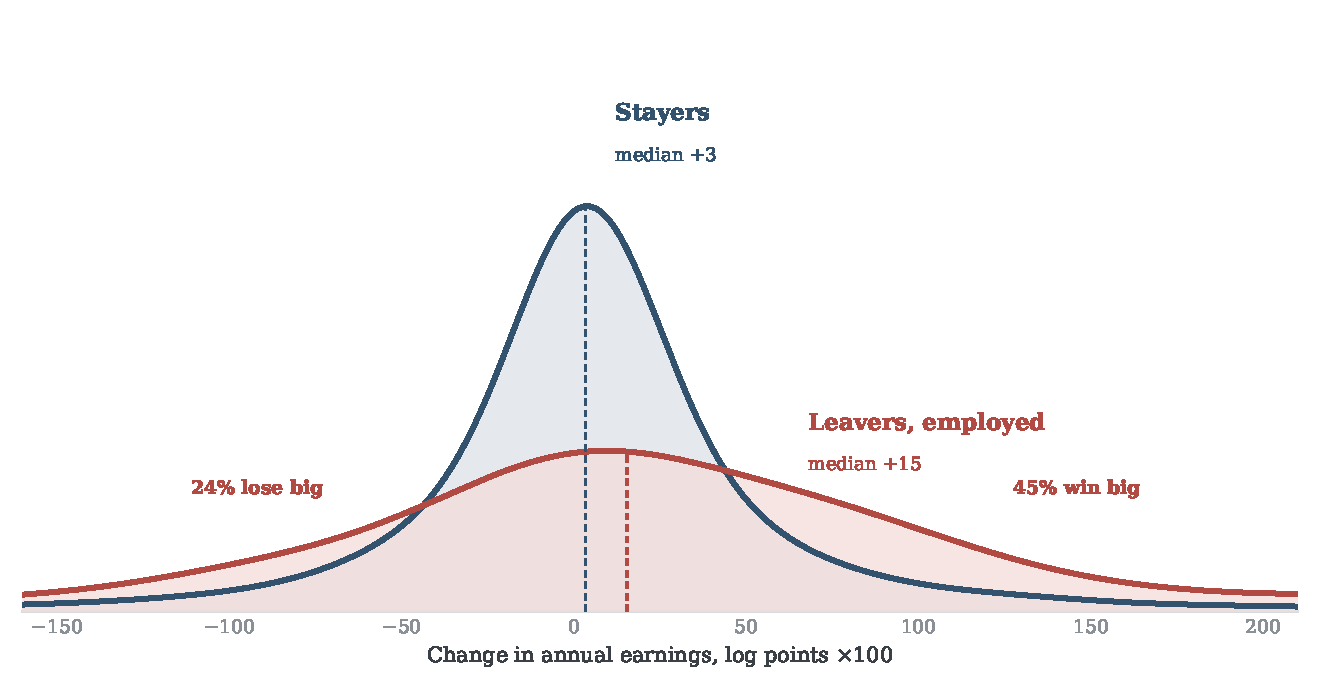
\includegraphics[height=0.66\textheight]{figures/g5b_earnings_density.pdf}
  \end{center}
  \vspace{-0.3em}
  {\small \msg{Message.} For employed leavers the earnings change is a gamble: a quarter lose big, nearly half win big.}\\[0.15em]
  {\small {\color{burg}\bfseries Policy.} Leaving buys risk, not a sure raise.}
\end{frame}

\begin{frame}{Pension coverage and leaving, across states}
  \begin{center}
    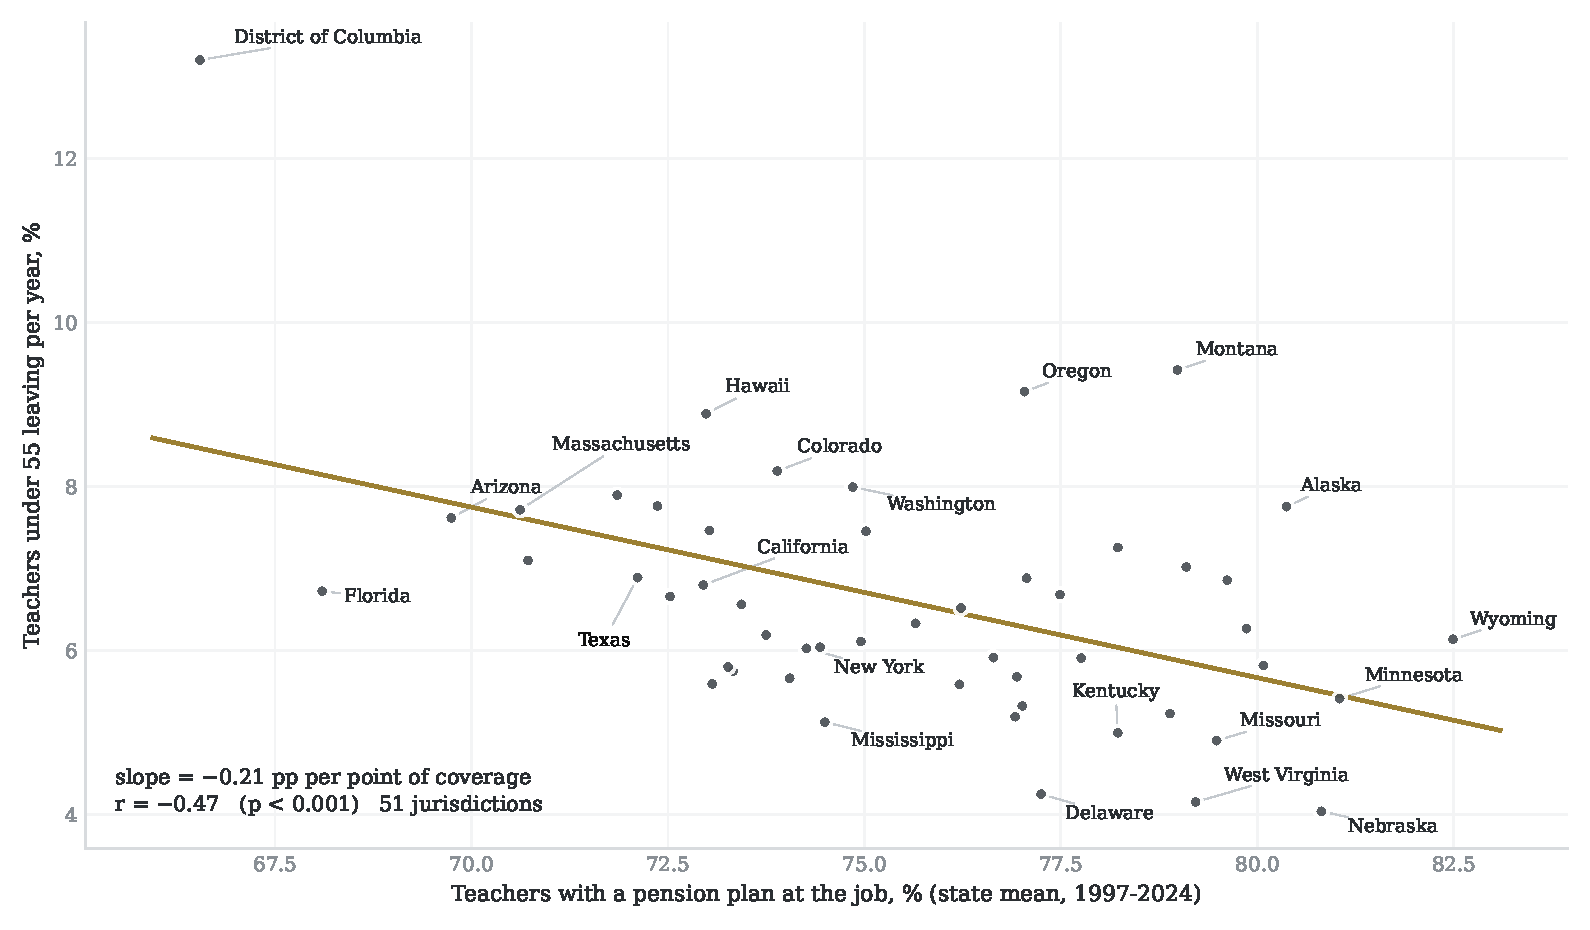
\includegraphics[height=0.66\textheight]{figures/pension_scatter_deck.pdf}
  \end{center}
  \vspace{-0.3em}
  {\small \msg{Message.} Where pension coverage is higher, fewer teachers under 55 leave: 0.21 points per point of coverage.}\\[0.15em]
  {\small {\color{burg}\bfseries Policy.} Pension design is a measurable retention margin.}
\end{frame}

% ================= Conclusion =================
\begin{frame}{Conclusion}
  \vspace{0.6em}
  \begin{itemize}\setlength\itemsep{1.2em}
    \item A labour force survey can measure teacher attrition at the person
          level, yearly, over three decades, and it replicates the official
          picture of the workforce.
    \item The definition of a leaver is a first-order choice: the same
          records yield rates from 5 to 19 percent per year.
    \item What the data say: attachment, pay and pensions, and life-cycle
          events correlate with leaving; demographics much less.
    \item The design travels: the same construction is feasible in the
          labour force surveys of Italy, Germany, the UK, France, Spain,
          Brazil and Mexico.
  \end{itemize}
\end{frame}

\end{document}
